\documentclass[]{book}
\newcommand\hmmax{0}
\newcommand\bmmax{0}
\usepackage{booktabs}

%% Language and font encodings
\usepackage[english]{babel}
\usepackage[utf8x]{inputenc}
\usepackage[T1]{fontenc}
\usepackage{gensymb}
\usepackage{pdfpages}
\usepackage{mparhack}


\usepackage[bitstream-charter]{mathdesign}
\let\circledS\undefined
%% Sets page size and margins
\usepackage[a4paper,top=2cm,bottom=2cm,left=1cm,right=7cm,marginparwidth=5cm, marginparsep=1cm]{geometry}

\newtheorem{theorem}{Theorem}[section]
\newtheorem{corollary}{Corollary}[theorem]
\newtheorem{lemma}[theorem]{Lemma}
\newtheorem{definition}{Definition}[section]
\newtheorem{principle}{Principle}[section]

%% Useful packages
\usepackage{amsmath}
\usepackage{bm}
\usepackage[makeroom]{cancel}
\usepackage{enumitem}
\usepackage{listings}
\usepackage{multirow}
\usepackage{amssymb}
\usepackage{float}
\usepackage{graphicx}
\usepackage[colorinlistoftodos]{todonotes}
\usepackage[colorlinks=true, allcolors=blue]{hyperref}
\usepackage[final]{matlab-prettifier}
\usepackage{courier}
\usepackage{algorithm}
\usepackage[noend]{algpseudocode}
\usepackage[]{appendix}
\usepackage{wrapfig}
\usepackage[final]{matlab-prettifier}
\usepackage[final]{mathtools}

\renewcommand\labelitemi{$\bullet$}

\definecolor{codecol}{rgb}{0.94, 0.94, 0.94}
\definecolor{dgreen}{rgb}{0.1, 0.49, 0.1}

\newcommand{\ea}{\nonumber \\}
\lstset{basicstyle=\footnotesize\ttfamily,breaklines=true}
\lstset{framextopmargin=50pt,frame=bottomline}

\newcommand{\norm}[2]{\left\Vert#1\right\Vert_{#2}}
\newcommand{\question}[1]{{\color{red}\textbf{Question: }\emph{#1}}}
\newcommand{\action}[1]{{\color{blue}\textbf{Action: }\emph{#1}}}
\newcommand{\epdp}{$(\epsilon, \delta)$-DP}
\newcommand{\alg}{$\mathcal{A}$}
\newcommand{\data}{$\mathcal{D}$}
\newcommand{\vect}[1]{\boldsymbol{\mathbf{#1}}}
\newcommand{\normaldist}[2]{$\mathcal{N}(#1, #2)$}
\newcommand{\expt}[2]{\mathbb{E}_{#2}[#1]}
\newcommand{\prob}[2]{\mathbb{P}_{#2}[#1]}
\newcommand{\model}[1]{\mathcal{M}_{#1}}
\newcommand{\indep}{\raisebox{0.05em}{\rotatebox[origin=c]{90}{$\models$}}}
\newcommand{\mset}[3]{\lbrace {#1}_{#2} \rbrace_{#2=1}^{#3} }
\DeclarePairedDelimiter{\ceil}{\lceil}{\rceil}
\DeclarePairedDelimiter\floor{\lfloor}{\rfloor}

\newcommand{\ix}[1]{%
  \leavevmode % if at the start of a paragraph
  \marginpar{\small\emph{#1}}% the note
}

\newcommand{\qx}[1]{%
	\leavevmode % if at the start of a paragraph
	\marginpar{\color{blue}\small\emph{#1}}% the note
}
\newcommand{\marfig}[2]{
  \marginpar{ \includegraphics[width=\marginparwidth]{#1} \centering \text{\small #2} }
}

\DeclareMathAlphabet{\altmathcal}{OMS}{cmsy}{m}{n}

\title{\textbf{4F5:  Advanced Information Theory \& Coding}\\
\textit{Course Notes}
}
\author{Mrinank Sharma}

\begin{document}
%\maketitle
%% \tableofcontents
%Please note that the margins of these notes can be used to check factual recall simply by covering up the right hand text.

\chapter{Information Theory and Statistics}
\section{Preliminaries}
\ix{Entropy}The entropy of a discrete random variable, $X$, with distribution $P$ on alphabet $\altmathcal{A}$ is defined as:
	\begin{align}
	H[X] = \expt{- \log P(X)}{X}
	\end{align}
\ix{Relative Entropy}The relative entropy between two distributions, $P$ and $Q$, is defined as:
\begin{align}
D(P||Q) = \sum_{a \in A} P(a) \log \frac{P(a)}{Q(a)}
\end{align}
\ix{Weak Law of Large Numbers}Let $X_1, X_2, \ldots$ be a sequence of iid random variable with mean $\mu$ and let $S_n = \frac{1}{n} \sum_{i=1}^{n} X_i$. Then, for any $\epsilon > 0$:
\begin{align}
\lim_{n \rightarrow \infty} P(|S_n - \mu| \geq \epsilon) = 0. 
\end{align}
Thus $S_n$ converges \emph{in probability} to $\mu$. \qx{Prove this, starting from Markov}.

If the sequence of random variables have a common distribution defined by probability mass function, $P$, the \ix{AEP}\emph{Asymptotic Equipartition Property (AEP)} states that the probability of a random string decays exponentially with $n$ with rate given by the entropy:
\begin{align}
\lim_{n \rightarrow \infty} (|\frac{-1}{n} \log P^{n}(X_1^n) - H[X]| \geq \epsilon) = 0
\end{align}
The AEP follows from the weak law of large numbers directly. Equivalently, $P^{n}(X_1^n) \simeq 2^{-n H[X]}$ for large $n$ with high probability. \qx{Try bounding the size of the typical set. } The typical set of strings for some $\epsilon$ is defined as:
\begin{align}
A_{\epsilon, n} = \lbrace 2^{-n(H[x] + \epsilon)} \leq x_1^n : P^n(x_1^n) \leq 2^{-n(H[x] - \epsilon)} \rbrace
\end{align}

\section{Fixed-Rate Lossless Data Compression}
\ix{Fixed-Rate Code} For a source $\vect{x} = \lbrace X_n \rbrace$, A fixed-rate lossless compression code consists of a sequence of codebooks $\lbrace B_n \rbrace$, where each $B_n$ is a set of source strings of length $n$. 

A simple way of implementing such a code, assuming that both encoder and decoder have access to the codebooks is by, for some message $x_1^n$:
\begin{enumerate}
	\item If $x_1^n \in  B_n$, send a $1$ followed by an index, taking $1 + \ceil{\log |B_n|}$ bits.
	\item If $x_1^n \notin  B_n$, send a $0$ followed by the uncompressed message, taking $1 + \ceil{\log |A^n|}$ bits.
\end{enumerate}
The rate and error probability of this code are:
\begin{align}
R_n = \frac{1}{n} (1 + \ceil{\log |B_n|}) \text{ bits / symbol} \hspace{0.5cm} P_e^{(n)} = Pr(X_1^n \notin B_n)
\end{align}
\begin{theorem}[Fixed Rate Coding Theorem]
	\ix{Fixed Rate Coding Theorem}For a memoryless source $\vect{X}$ with entropy $H[X_i]$:
	\begin{enumerate}[label=(\alph*): ]
		\item For any $\epsilon >0$, there exists some fixed-rate code $\lbrace B_{n}^* \rbrace$ with vanishing error of probability $P_e^{(n)} \rightarrow 0$ as $n \rightarrow \infty$ with rate:
		\begin{align}
		R_n \leq H[X] + \epsilon + \frac{2}{n}
		\end{align}
		for all $n$.
		\item Let $\lbrace B_{n} \rbrace$ be a fixed-rate code with $P_e^{(n)} \rightarrow 0$ as $n \rightarrow \infty$. Then, for any $\epsilon > 0$:
		\begin{align}
		R_n \geq H[X] - \epsilon
		\end{align}
		eventually.
	\end{enumerate} 
\end{theorem}
\qx{Prove the Fixed Rate Coding Theorem}(a) can be proved by taking $B_n^*$ to be the set of typical sequences and using the AEP. To prove (b), note that
\begin{align}
P^n(B_n \cap B_n^{*}) &= P^n(B_n) + P^n(B_n^*) - P^n(B_n \cup B_n^*) \nonumber \\
&= 2 - P_e^{(n)} - P_*^{(n)} -  P^n(B_n \cup B_n^*) \nonumber \\
&\geq 1 - P_e^{(n)} - P_*^{(n)}
\end{align}
where $P_e^{(n)}$ is the error for some code with vanishing error probability and $P_*^{(n)}$ is the error for code defined by the typical set. Note that the above error probabilities are vanishing. Thus, eventually, $P^n(B_n \cap B_n^{*}) > \frac{1}{2}$ which combined with typical inequalities used when considering the typical set, produces the desired result. 

If a rate-optimal code is desired i.e. the asymptotic rate is exactly equal to the entropy, the error probability can be exponentially small i.e. $P_e^{(n)} \simeq 2^{-nD^{*}}$ and it is possible to calculate the largest possible value of $D^*$. \action{Come back to this - what is this optimal value!}

\section{Hypothesis Testing}
A simple hypothesis test is considered: given data $x_1^n$ produced by some memoryless source and two candidate distributions, $P$ and $Q$ on the finite alphabet $A$, we must decide whether the data was produced by $P$ or $Q$. Any hypothesis test can be computing some region, $B_n \in A^n$ in which, if the data is lies in this region, we declare $P$ and otherwise $Q$ is declared. We seek to choose $B_n$ to minimise the error probability. 
\begin{align}
e_1^{(n)} &= Pr(\text{declare } P| X_1^n \sim Q^n ) = Q^n(B_n) \\
e_2^{(n)} &= Pr(\text{declare } Q| X_1^n \sim P^n ) = P^n(B_n^{c})
\end{align}
\ix{Error Probability: Tension}Note that the `cost' of these errors is often asymmetry i.e. a false negative could be far more significant than a false negative. There is a tension between this error probabilities; minimising $e_1^{(n)}$ requires making $B_n$ smaller but reducing $e_2^{(n)}$ requires making $B_n^c$ smaller. 

\begin{theorem}[Stein's Lemma]
	\ix{Stein's Lemma}Let $P$ and $Q$ be two different distributions over $A$ such that $D = D(P||Q)$ is neither $0$ nor $\infty$. Suppose that $\vect{X}$ is a memoryless source on $A$, distributed either to $P$ or $Q$. 
	\begin{enumerate}[label=(\alph*): ]
		\item For any $\epsilon > 0$, there is a hypothesis test with regions $\lbrace B_n^* \rbrace$ such that
		\begin{align}
		e_1^{(n)} \leq 2^{-n(D - \epsilon)}
		\end{align}
		for all $n$ and with $e_2^{(n)} \rightarrow 0$ as $n \rightarrow \infty$. 
		
		\item For a hypothesis test with regions  $\lbrace B_n \rbrace$ such that $e_2^{(n)} \rightarrow 0$ as $n \rightarrow \infty$, for any $\epsilon > 0$:
		\begin{align}
		e_1^{(n)} \geq 2^{-n(D + \epsilon + \frac{1}{n})}
		\end{align}
	\end{enumerate}
\end{theorem}
The average log likelihood ratio can be expressed as\qx{Prove Stein's Lemma. }
\begin{align}
\frac{1}{n} \log \frac{P^n(X_1^n)}{Q^n(X_1^n)} = \frac{1}{n} \sum_{i=1}^{n} \underbrace{\log \frac{P(X_i)}{Q(X_i)}}_{Z_i} \xrightarrow{P} D(P || Q)
\end{align}
The weak law of large numbers thus states that the above sum convergences in probability to the mean of $Z_i$, which (under $P$), is $D(P || Q)$. The likelihood-ratio typical set can be defined as:
\begin{align}
B_n^* = \Big\lbrace x_1^n \in A^n: 2^{n(D - \epsilon)} \leq \frac{P^n(x_1^n)}{Q^n(x_1^n)} \leq 2^{n(D + \epsilon)}  \Big\rbrace
\end{align}
This can be used to prove (a), taking the decision regions defined by the likelihood-ratio typical set. (Note that these regions are asymptotically optimal but may not be optimal for finite n; this proof is only about existence however). A bound on $e_1^{(n)}$ is obtained by applying typical bounds related to typical sets. The proof of part (b) follows the same format as for the fixed rate coding theorem. 

\ix{Are the assumptions valid?}Note that the assumptions that $D \neq 0$ is trivial, as it is equivalent to assuming that $P$ and $Q$ are different distributions. Assuming that $D \neq \infty$ means that every symbol possible under distribution $P$ is also possible under $Q$; if this wasn't true, it would be very easy to perform the hypothesis test (e.g. waiting until we see symbols in one alphabet but not the other). 

\ix{Interpret Stein's Lemma}Stein's lemma tells that if one of the error probability vanishes, the fastest rate at which the other error can decrease is given by $D(P||Q)$. Thus the larger the `distance' between $P$ and $Q$, the fewer data points are required to give a certain error probability and the easier it is to distinguish between the distributions. This motivates the interpretation of the relative entropy as a natural distance measure for discrete distributions. 

\begin{theorem}[Neyman-Pearson Lemma]
	\ix{Neyman-Pearson Lemma} For a hypothesis test between two distributions, $P$ and $Q$, based on $n$ data samples, consider the `likelihood-ratio' decision region:
	\begin{align}
		B_{NP} = \Bigg \lbrace x_{1}^n \in A^n : \frac{P^n(x_{1}^n)}{Q^n(x_{1}^n)} \geq T \Bigg \rbrace
	\end{align}
	for some threshold $T > 0$ with error probabilities:
	\begin{align*}
	e_{1, NP}^{(n)} = Q^n(B_{NP}) \hspace{1cm} e_{2, NP}^{(n)} = P^n(B_{NP}^c)
	\end{align*}
	This decision region is optimal in the following sense. For any other decision region, $B_n \subset A^n$, if one the error probabilities, $e_2^{(2)}$, is better than that of $B_{NP}$, then the other one is worse:
	\begin{align*}
	e_2^{(n)} \leq e_{2, NP}^{(b)} \Rightarrow e_1^{(n)} \geq e_{1, NP}^{(b)}
	\end{align*}
\end{theorem}
\qx{Prove the Neyman-Pearson Lemma}\textbf{Proof: } Note the following inequality always holds:
\begin{align}
\Big[ \mathbb{I}_{B_{NP}}(x_1^n) - \mathbb{I}_{B_{n}}(x_1^n) \Big]\Big[ P^n(x_1^n )- TQ^n(x_1^n)\Big] \geq 0
\end{align}
It can be seen that this inequality holds simply by considering possible regions which $x_1^n$ may be in. Then summing over all $x_1^n \in A^n$ yields, substituting and rearranging yields the desired result. 

\ix{Empirical Distribution}The empirical distribution induced by $x_1^n$ on $A^n$ is simply the empirical frequencies with with $a$ appears in $x_1^n$. Formally:
\begin{align}
\hat{P}_n(a) = \frac{1}{n} \sum_{i=1}^{n} \mathbb{I}_{\lbrace a \rbrace}(x_i)
\end{align}

\ix{Relative Entropy Formulation}The Neyman-Pearson decision region can equivalent be expressed as:
	\begin{align}
B_{NP} = \Big \lbrace x_{1}^N \in A^n : D(\hat{P}_n || Q)\geq D(\hat{P}_n || P) + T' \Big \rbrace
\end{align}
with $T' = \frac{1}{n} \log T$. Informally, this test computes the empirical distribution and chooses $P$ if the distribution is closer to $P$ (including a margin).\qx{Prove the following line} By expanding the form for the logarithm of the likelihood, it can be shown that:
\begin{align*}
\log \frac{P^n(x_{1}^n)}{Q^n(x_{1}^n)} = n [D(\hat{P}_n || Q) - D(\hat{P}_n || P)]
\end{align*}
from which the reformulation directly follows. 

\section{Relative Entropy and Convexity}
\ix{Convexity and Concavity} Let $F: E \rightarrow \mathbb{R}$ be a function defined on the convex set $E \subset \mathbb{R}^n$. Then:
\begin{enumerate}
	\item $f$ is convex if, for every pair of points, $x, y \in E$ with $x\neq y$, and every $\lambda \in [0, 1]$, 
	\begin{align}
	f(\lambda x + (1-\lambda)y) \leq \lambda f(x) + (1-\lambda)f(y)
	\end{align}
	\item $f$ is concave if the inequality above is reversed, or equivalently if $-f$ is convex. 
\end{enumerate}
A function is \emph{strictly} convex/concave if the above inequality is strict. \qx{Prove link between convexity and the second derivative}Convex functions have a positive second derivative, and a strictly positive second derivative implies strict convexity.
\begin{theorem}[Jensen's Inequality]
	For\ix{Jensen's Inequality} any convex function $f: R \rightarrow \mathbb{E}$ and any RV, $X$, taking values in $E$:
	\begin{align}
	f(\expt{X}{}) \leq \expt{f(X)}{}
	\end{align}
	If $f$ is strictly convex, equality is achieved iff $X$ is constant. 
\end{theorem}

\begin{theorem}[Log-Sum Inequality]
	For\ix{Log-Sum Inequality} arbitrary non negative constants, $\lbrace a_i, b_i \rbrace_{i=1}^n$, 
	\begin{align}
	\sum_i a_i \log \frac{a_i}{b_i} \geq \Big( \sum_i a_i \Big) \log \frac{\sum_i a_i }{\sum_i b_i }
	\end{align}
	Equality is achieved if the ratios $a_i / b_i$ are the same $\forall i$. 
\end{theorem}
\qx{Prove the Log-Sum Inequality} Let $A = \sum_i a_i$ and $B = \sum_i b_i$. Define a random variable, $X$ as follows:
\begin{align}
X = \frac{a_i}{b_i} \text{ with probability } \frac{b_i}{B} \forall i \nonumber
\end{align}
Let $f(x) = x\log x$ with the convention that $f(0) = 0$, and note this is a strictly convex function.  Simply applying Jensen's inequality, and considering the condition for equality in Jensen's inequality yields the desired result. 

\begin{theorem}[Data Processing Inequality]
	Let\qx{Prove the Data Processing Inequality} $X \sim P_X$ and $X' \sim Q_X$ be two RVs over the same alphabet, $A$, defined by their PMFs. Let $f: A \rightarrow B$ be an arbitary function, and denote the corresponding output PMFs as $P_{f(X)}$ and $Q_{f(X)}$. Then:
	\begin{align}
	D(P_{f(X)} || Q_{f(X)}) \leq D(P_X|| Q_X)
	\end{align}
	i.e. data processing cannot possibly make the two distributions more distinguishable. 
\end{theorem}
The proof is straightforward by applying the log-sum inequality and writing the transformed distributions. 

\begin{definition}[Total Variation]
	The total variation distance between two PMFs, $P$ and $Q$, defined on the same alphabet, $A$, is
	\begin{align}
	||P - Q||_{TV} = \sum_{x\in A} | P(x) - Q(x) |
	\end{align}
\end{definition}
\ix{Alternative Total Variation Interpretation}Define the set $B = \lbrace x \in A: P(x) > Q(x) \rbrace$. The total variation can alternatively be interpreted as:
\begin{align}
	||P - Q||_{TV} = 2 (P(B) - Q(B))
\end{align}
The proof of the above is straightforward, and follows by definition of the set $B$. 

\begin{theorem}[Pinsker's Inequality]
	\ix{Pinsker's Inequality}For any two PMFs, $P$ and $Q$, on the same alphabet, $A$, 
	\begin{align}
	||P - Q||_{TV}^2 \leq (2 \ln 2) D(P || Q) 
	\end{align}
\end{theorem}

\qx{Pinsker's Inequality: Bernouli Proof}Consider $P = \text{Bern}(p)$ and $Q = \text{Bern}(q)$. Without loss of generality, it can be assumed that $q \leq p$, since otherwise labels can be exchanged. Define:
\begin{align}
\Delta(p, q) = (2 \ln 2) D(P || Q) - ||P - Q||_{TV}^2
\end{align}
Pinsker's inequality can be proved for this case by showing that $\Delta(p, q) > 0$. Since $\Delta(p, p) = 0$, this is equivalent to showing that:
\begin{align*}
\frac{\partial \Delta(p, q)}{\partial q} \leq 0
\end{align*}
since $q$ would be decreased from $p$. For the Bernoulli case, this can be shown by substituting in, expanding and considering the bounds on $q$ and $p$. 

\ix{How to expand to general random variables} For general random variables, the data-processing inequality is applied with $f(x) = \mathbb{I}_{B} (x)$ with $B = \lbrace x \in A: P(x) > Q(x) \rbrace$. Then, if $X \sim P$ and $X' \sim Q$, $f(X) \sim \text{Bern}(P(B))$ and $f(X') \sim \text{Bern}(Q(B))$, and $Q(B) \leq P(B)$. Then, applying the data processing inequality:
\begin{align}
(2 \ln 2) D(P || Q) &\geq  (2 \ln 2) D(P_f || Q_f) \nonumber \\ 
&\geq ||P_f - Q_f||_{TV}^2 \nonumber \\
&= (2(P(B) - Q(B)))^2 \nonumber \\
&= || P - Q||_{\text{TV}}^2
\end{align} 

\begin{theorem}[Convexity of Relative Entropy]\ix{Convexity of Relative Entropy}The relative entropy, $D(P || Q)$, is jointy convex. For any $P_1, P_2, Q_1, Q_2$ and $\lambda \in [0, 1]$:
	\begin{align}
	D(\lambda P_1 + (1-\lambda)P_2 || \lambda Q_1 + (1-\lambda)Q_2) \leq \lambda D(P_1 || Q_1) + (1-\lambda) D(P_2 || Q_2) 
	\end{align}
\end{theorem}
The proof for the above is similar to the proof of the data-processing inequality. \qx{Prove Convexity}.

Note that if $P$ is a distribution on an alphabet, $A$, and $U$ is the uniform distribution over $A$, then:
\begin{align}
D(P || U) = \log |A| - H[P]
\end{align}
This, with the convexity of relative entropy, directly implies that the following corollary. 
\begin{corollary}[Concavity of Entropy]
	The entropy, $H[P]$, is a concave function on the set of all PMFs, $P$, on a finite alphabet. 
\end{corollary}

\section{Poisson Approximation}
\textbf{Note: } In this section, it is convenient to use entropies defined by the natural log, denoted by subscript $e$.

\ix{Binomial to Poisson}Suppose that $\lambda$ events, on average, occur in some time window. Let $X_1, \ldots, X_n$ be a sequence of RVs with $X_i \stackrel{iid}{\sim} \text{Bern}(\frac{\lambda}{n})$. Then, their sum converges to a Poisson distribution.
\begin{align}
Pr(S_n = k) \stackrel{n \rightarrow \infty}{\rightarrow} \exp [-\lambda] \frac{\lambda^k}{ k!}
\end{align}
In general, let $\lbrace X_i \rbrace_{i=1}^N$ be a sequence of RVs with $X_i \sim \text{Bern}(p_i)$. Then, the distribution of the sum of the RVs, $S_n$ is close to $\text{Po}(\lambda)$ with $\lambda = \expt{S_n}{}$, provided that each $p_i$ is `small' and the $X_i$ are `weakly' dependent. 

\begin{theorem}[Poisson Approximation I]
	Suppose $S_ n = X_1 + \cdots + X_n$ with $X_i \stackrel{iid}{\sim} \text{Bern}(p_i)$. Then
	\begin{align}
	D_e(P_{S_n} || \text{Po}(\lambda)) \leq \sum_i p_i^2
	\end{align}
	with $\lambda = \expt{S_n}{} = \sum_i p_i$. 
\end{theorem}
\qx{Show this proves the Binomial-to-Poisson Convergence}Note that this theorem implies the binomial-to-Poisson convergence. Additionally, this theorem is not asymptotic and we form an equality that holds for all $n$. It also provides an easily computable, quantitative bound on the difference between $P_{S_n}$ and the limiting Poisson distribution, without assuming that each $p_i$ is equal. 

\begin{theorem}[Poisson Approximation II]
	Suppose $S_ n = X_1 + \cdots + X_n$ with $X_i \sim \text{Bern}(p_i)$, allowing dependence between the Bernoulli RVs. Then
	\begin{align}
	D_e(P_{S_n} || \text{Po}(\lambda)) \leq \sum_i p_i^2 + \sum_i H_e[X_i] - H_e(X_1^n)
	\end{align}
	with $\lambda = \expt{S_n}{} = \sum_i p_i$. 
\end{theorem}
\ix{Poisson Proof}\textbf{Proof:} $A = \lbrace 0, 1, \ldots \rbrace$ and $Z_i \stackrel{iid}{\sim}\text{Po}(p_i)$, meaning that the distribution of the sum $T_n =  \sum_i Z_i$ is $\text{Po}(\lambda)$. Define $f: A^n \rightarrow A$ as follows:
\begin{align}
f(x_1^n) = \sum_{i=1}^n x_i 
\end{align}
meaning that $S_n = f(X_1^n)$ and $T_n = f(Z_1^n)$. \qx{Poisson Approximation Proof}
\begin{align}
D_e(P_{S_n} || \underbrace{\text{Po}(\lambda)}_{P_{T_n}}) = D_e(P_{f(X_1^n)} || P_{f(Z_1^n)}) \leq D_e(P_{X_1^n} || P_{Z_1^n})
\end{align}
Next, note that for every $p \in [0, 1]$:
\begin{align}
D_e(\text{Bern}(p)|| \text{Po}(p)) \leq p^2
\end{align}
Substituting in for the definition of relative entropy, and multiplying and dividing by the product of the marginal distributions yields the desired result. 

This results gives a precise quantitative definition of what small $p_i$ corresponds to i.e. $p_i$ must be small enough to have a small sum of squares. Additionally, `weakly dependent' is also quantified. Note that the term $\sum_i H_e[X_i] - H_e(X_1^n)$ is non-negative and only $0$ if independent. 

\section{Estimation and Information}
\ix{Problem Setup}IID data, $X_1^n$ is generated by some unknown distribution, $P$, which is assumed to belong to some parametric family of distributions, $\altmathcal{P} = \lbrace P_\theta: \theta \in \Theta \rbrace$. The parameter space, $\Theta$, is usually some interval of real numbers or a subset of $\mathbb{R}^d$. Assume that the true distribution lies within this parameter space, $P = P_{\theta^*}$. We hope to find a good estimator for $\theta^*$, $\hat{\theta} = \hat{\theta}(X_1^n)$. Note that this estimator is a function of the data i.e. $\hat{\theta}: A^n \rightarrow \Theta$, and it is a random variable. 

\ix{Bias-Variance Tradeoff}A reasonable approach is to try and minimise the mean squared error. 
\begin{align}
\text{MSE}(\hat{\theta}; \theta) &= \expt{(\hat{\theta} - \theta)^2}{P_\theta} \nonumber\\
&= \underbrace{\expt{(\hat{\theta} - \expt{\hat{\theta}}{P_\theta})^2}{P_\theta}}_{\text{var}[\hat{\theta}]} + \underbrace{(\expt{\hat{\theta} -\theta}{P_\theta})^2}_{\text{bias}(\hat{\theta}; \theta)^2}
\end{align}
In order to have a small mean squared error, we need both a small bias and small variance. Typically, there is a tension between the two terms known. 

\subsection{Unbiasedness and Maximum Likelihood}
It may seem sensible to restrict attentions to unbiased estimators and choose the estimator with the smallest possible variance, but in certain cases (such as for the entropy), unbiased estimators do not exist or may lead to implausible estimates. 

\ix{Maximum Likelihood}The \emph{Maximum Likelihood Principle} states that the best estimate is given by the parameter that maximises the likelihood of the data:
\begin{align}
\hat{\theta}_{\text{MLE}} &= \arg \max_{\theta \in \Theta} P_\theta^n(x_1^n) \\
&= \arg \min_{\theta \in \Theta} D(\hat{P}_n|| P_\theta)
\end{align}
\qx{Proof: MLE and Relative Entropy}The MLE estimate can equivalently be expressed as as the closest parametric distribution to the empirical distribution. This can be proved  by rewriting the negative log-likelihood. 

\subsection{Fisher Information}
When forming maximum likelihood estimates, the relative entropy is differentiated with respect to $\theta$. The behaviour of the relative entropy, $D_e(P_\theta || P_{\theta'})$, is now investigated for $\theta$ close to $\theta'$. Define $\Delta(x) = P_\theta(x) - P_{\theta'}(x)$. 
\begin{align}
D_e(P_\theta || P_{\theta'}) &= \sum_x (P_{\theta'}(x) + \Delta(x)) \ln \Bigg[1 + \frac{\Delta (x)}{P_{\theta'}(x)}\Bigg] \nonumber \\
&\simeq \sum_x (P_{\theta'}(x) + \Delta(x)) \Bigg[\frac{\Delta (x)}{P_{\theta'}(x)} -\frac{1}{2} \Bigg( \frac{\Delta (x)}{P_{\theta'}(x)}\Bigg) ^2 \Bigg] \nonumber \\
&\simeq \frac{1}{2} \sum_x P_{\theta'}(x) \Big( \frac{P_{\theta}(x) - P_{\theta'}(x)  }{P_{\theta'}(x)}\Big)^2 \nonumber
\end{align}
assuming that $\theta - \theta'$ is small and thus that $\Delta$ is small and noting that $\sum_x \Delta(x) = 0$. Then, assuming that the derivatives of $P_\theta(x)$ exist with respect to $\theta$, $P_\theta(x) - P_{\theta'}(x) \simeq (\theta - \theta')P_\theta'$. Therefore:
\begin{align}
D_e(P_\theta || P_{\theta}') \simeq \frac{1}{2} (\theta - \theta')^2 \mathbb{E}\ \Bigg[ \Big(\frac{P'_{\theta}(X)}{P_\theta(X)}\Big)^2 \Bigg]
\end{align} 
Thus $D_e(P_\theta || P_{\theta}')$ is locally quadratic in $\theta$.

\begin{definition}[Fisher Information]
	\ix{Fisher Information}Let $\altmathcal{P} = \lbrace P_\theta: \theta\in [a, b] \rbrace$ be a one-dimensional parametric family such that the derivatives $P_\theta'$ of $P_\theta$ with respect to $\theta$ exist for all $\theta\in [a, b]$. The Fisher Information, $J(\theta)$, for this parametric family is defined as:
	\begin{align}
	J(\theta) = \mathbb{E}_{P_\theta}\ \Bigg[ \Big(\frac{P'_{\theta}(X)}{P_\theta(X)}\Big)^2 \Bigg]
	\end{align}
\end{definition}
\ix{Alternative Fisher Information Expressions}The Fisher Information can also be expressed as:\begin{align}
	J(\theta) = \mathbb{E}_{P_\theta}\ \Bigg[ \Big(\frac{\partial}{\partial\theta} \lbrace \ln P_{\theta}(X) \rbrace \Big)^2 \Bigg]
	\end{align} 
Alternatively:\qx{Show Alternative Expression}
\begin{align}
	J(\theta) = \text{var}_{P_\theta}\ \Bigg[ \underbrace{\frac{\partial}{\partial\theta} \lbrace \ln P_{\theta}(X) \rbrace  \Bigg]}_{\rho(\theta; X)}
	\end{align} 
where $\rho(\theta; X)$ is known as the score function. To prove, consider the mean of the score function. 

\begin{theorem}[Cramér-Rao Bound for Any Estimator]
	\ix{Cramér-Rao Bound}The MSE of any estimator, $\hat{\theta}$, satisfies:
	\begin{align}
	\text{var}_{P_\theta}(\hat{\theta}) \geq \frac{[1 + \text{bias}'(\hat{\theta}; \theta)]}{J(\theta)}
	\end{align}
	where $\text{bias}'(\hat{\theta}; \theta)$ is the derivative of the bias with respect to $\theta$. 
\end{theorem}
For an unbiased estimator, the derivative of the bias is zero. 

\qx{Cramér-Rao Bound Proof}\textbf{Proof}: Consider the following:
\begin{align}
J(\theta)\ \text{var}_{P_\theta}(\hat{\theta}) = \text{var}_{P_\theta}(\rho(\theta; X))\ \text{var}_{P_\theta}(\hat{\theta}) \leq \mathbb{E} \Bigg[ (\rho(\theta; X) - \underbrace{\expt{\rho(\theta; X)}{P_\theta}}_{0}) (\theta(X) - \expt{\hat{\theta}}{P_\theta})\Bigg]
\end{align}
since the correlation coefficient between two RVs is bounded by $1$ i.e.
\begin{align}
\text{corr}(X, Y) = \frac{\text{cov}(X, Y)}{\sqrt{\text{var}(X) \text{var}(Y)}} = \frac{\expt{(X - \expt{X}{})(Y - \expt{Y}{})}{}}{\sqrt{\text{var}(X) \text{var}(Y)}} \leq 1
\end{align}
\qx{Proof: Fisher Information for IID Samples}Suppose that $X_1^n$ is IID according to some distribution, $P_\theta$. It can be shown that:
\begin{align}
J_n(\theta) = nJ(\theta)
\end{align}
This is straightforward to show by the independence of each datapoint. This gives a natural extension of the Cramér-Rao Bound. 

\chapter{Practical Number Theory \& Algebra}
\section{Number Theory}
\begin{theorem}[Euclid's Division Theorem]
	\ix{Euclid's Division Theorem}For any integers $n, d \neq 0$ there exist unique integers, $q, r$ such that:
	\begin{align}
	n = qd + r \text{ with } 0 \leq r < |d|
	\end{align}
\end{theorem}
\qx{Proof Outline}This theorem can be shown by showing that there exists a pair, $(q', r')$ with $n=qd+r$, and that this can be used to recursively generate pairs until one is found which satisfies the condition. Additionally, it is shown that this pair is unique (try showing this yourself). 

\begin{theorem}[Properties of Remainders]
	\ix{Properties of Remainders}Renote the remainder of $n$ when it is divided by $d$ as $R_d(n)$. Remainders have the following properties:\qx{Try proving these!}
	\begin{enumerate}
		\item $R_d(n + kd) = R_d(n)$
		\item $R_d(k + n) = R_d(R_d(k) + R_d(n))$
		\item $R_d(kn) = R_d(R_d(k)\cdot R_d(n))$
	\end{enumerate}
\end{theorem}

\begin{definition}[Greatest Common Divisor]
	The greatest common divisor between integers $n_1, n_2$ is the largest integer $d$ which divides both $n_1$ and $n_2$. Denote the greatest common divisor as $\text{gcd}(n_1, n_2)$. 
\end{definition}
Note that signs are irrelevant for the GCD. 

\begin{theorem}[Fundamental Property of GCDs]
	For any integers, $n_1, n_2$ and $k$:
	\begin{align}
	\text{gcd}(n_1 + k n_2, n_2) = \text{gcd}(n_1, n_2)
	\end{align}
\end{theorem}
Any number that divides both $n_1$ and $n_2$ will also divide $n_1 + kn_2$ by the property of remainders, giving us this fundamental property. 

\ix{Euclid's Algorithm}Imagine picking $k$ as the negative quotient of $n_1 / n_2$. Then, the above property implies that:
\begin{align}
\text{gcd}(n_1, n_2) = \text{gcd}(R_{n_2}(n_1), n_2)
\end{align}
which provides an algorithm for computing the GCD of two numbers:
\begin{enumerate}
	\item Label the numbers such that $n_1 > n_2$. 
	\item Compute $r = R_{n_2}(n_1)$ and assign $n_1 \leftarrow n_2$, $n_2 \leftarrow r$. 
	\item If $n_2 = 0$, terminate and output $n_1$. Otherwise, repeat.
\end{enumerate}

\begin{theorem}[Even \& Odd Properties of GCDs]
	For any integers, $n_1$ and $n_2$:
	\begin{enumerate}
		\item If $n_1, n_2$ are both even, then $\text{gcd}(n_1, n_2) = 2\ \text{gcd}(n_1/2, n_2/2)$.
		\item If $n_1$ is even and $n_2$ is odd, then $\text{gcd}(n_1, n_2) = \text{gcd}(n_1/2, n_2)$.
		\item If $n_1, n_2$ are odd, then $\text{gcd}(n_1, n_2) = \text{gcd}(\frac{n_1 - n_2}{2}, n_2)$. 
	\end{enumerate}
\end{theorem}
\ix{Stein's Algorithm}Applying the above properties gives \emph{Stein's Algorithm} which is more efficient that Euclid's algorithm. 

\begin{theorem}[Greatest Common Divisor Theorem]
	For any integers $n_1$ and $n_2$ not both zero, there exist (not necessarily unique) integers such that:
	\begin{align}
	\text{gcd}(n_1, n_2) = a n_1 + b n_2
	\end{align}
\end{theorem}
\qx{Try Proving this Yourself}The proof of this theorem considers $d' = an_1 + bn_2$ which is defined as the smallest possible integer combination of $n_1$ and $n_2$. It can be shown that $d'$ divides both $n_1$ and $n_2$ exactly, but also that the GCD divides $d'$, meaning that $d'$ must be the GCD. In many cases, we are very interested in calculating the values of $a$ and $b$. 

\ix{Extended Euclid's Algorithm}Both Stein's Algorithm and Euclid's algorithm can be extended to also compute the pair $(a, b)$. The key idea is to maintain two pairs $(a_1, b_1)$ and $(a_2, b_2)$ such that, after $k$ iterations:
\begin{align}
a_1^{(k)} n_1 ^{(0)} + b_1^{(k)} n_2^{(0)} &= n_1^{(k)} \\
a_2^{(k)} n_1 ^{(0)} + b_2^{(k)} n_2^{(0)} &= n_2^{(k)} 
\end{align}
The pairs are initialised as $(a_1^{(0)}, b_1^{(0)}) = (1, 0)$ and $(a_2^{(0)}, b_2^{(0)}) = (0, 1)$.\qx{Show Recursive Relationships} For Euclid's algorithm, the following recursive relationships hold:
\begin{align}
a_1^{(k+1)} &= a_2^{(k)} \\
b_1^{(k+1)} &= b_2^{(k)} \\
a_2^{(k+1)} &= a_1^{(k)} - qa_2^{(k)} \\ 
b_2^{(k+1)} &= b_1^{(k)} - qb_2^{(k)} 
\end{align}
The algorithm ends by setting $(a, b) = (a_1, b_1)$ since $n_1^{(k^*)} = \text{gcd}(n_1^{(0)}, n_2^{(0)})$ and $n_2^{(k^*)} = 0$. 

A number, $p > 1$, is prime iff it is only divisible by $1$ and itself. If $n < p$, then $\text{gcd}(p, n) =1$. Note that two numbers are called co-prime if $\text{gcd}(n_1, n_2) = 1$. 

\begin{theorem}[Fundamental Theorem of Arithmetic]
	Every integer, $n>1$, is either prime or can be \textbf{uniquely} expressed as a product of prime numbers. 
\end{theorem}
Any non-prime number, can be expressed as a product of two integers less than the factor. This can be repeatedly endlessly for any non-prime factor, and given that there are a finite number of integers, that we can express any number as a product of primes. 

\ix{Uniqueness of Prime Decomposition}If $n$ has two distinct prime factorisations, either there is prime in one factorisation which is not present in the other or a factor appears an unequal number of times in each factorisation. Denote the unique factor as $p'$. $p'$ must divide $n$, meaning that it must divide one of the factors in the other factorisation or be expressible as a product of factors, meaning that $p'$ is not prime or one of the other factors is prime. If the factor $p'$ appears $k_1$ times in one factorisation and $k_2$ times in the other, the same argument can be made for $p^{\max(k_1, k_2)}$, meaning that the factorisation of primes must be unique. 

\begin{theorem}
	There are infinitely many primes. 
\end{theorem}

\begin{theorem}[Prime Number Theorem]
	For any integer, let $\pi(n)$ be the number of primes up to and including $n$. Then:
	\begin{align}
	\lim_{n\rightarrow \infty} \frac{\pi(n)}{n / \ln(n)} = 1
	\end{align}
	i.e. the number of primes grows roughly as $n / \ln n$
\end{theorem}

\begin{theorem}[Chinese Remainder Theorem]
	\ix{Chinese Remainder Theorem} Let $\lbrace m_i \rbrace_{i=1}^k$ be pairwise co-prime integers (or moduli). Let $m = \prod_i m_i$. Then, for any choice of residues, $\lbrace r_i \rbrace_{i=1}^k$ such that $0 \leq r_k < m_j$ there exists a \textbf{unique} non-negative integer, $n < m$, for which:
	\begin{align}
	R_{m_j}(n) = r_j
	\end{align}
	i.e. for co-prime moduli, the residues uniquely define a number. 
\end{theorem}
\qx{Uniqueness}Uniqueness can be shown by assuming there are two integers, $n$ and $n'$ which satisfy the condition. Considering $R_{m_j}(n - n')$ shows that $n-n'$ is divided by all the of relatively prime module, meaning that $n-n'$ can be expressed as some multiple of the product of the moduli. However, $n - n' < m$, meaning that $n - n' = 0$. 

\qx{Existence}There are $m$ choices for $n$ and there are $m = \prod_j m_j$ choices for the residue vector. Since each residue vector uniquely corresponds to a number, and each number has residues, there must be an integer for every choice of residues.

\ix{From Residues to $n$}It is clearly easy to calculate residues from a number $n$, but what about the other way around? Define $u_j = \frac{m}{m_j}$ and note that $\text{gcd}(u_j, m_j) = 1$ since all the moduli are co-prime. Then, we can write:
\begin{align}
\text{gcd}(m_j, u_j) = a_j m_j + b_j u_j = 1
\end{align}
Additionally, $R_{m_j}(a_j m_j + b_j u_j) = R_{m_j}(b_j u_j) = 1$. Then, $R_{m_j}(\alpha b_j u_j) = \alpha $ for $\alpha < m_j$. Also note that $R_{m_t}(b_j u_j) = 0$ since $m_t$ divides $u_t$. Therefore:
\begin{align}
n = R_m \big[  \sum_{j=1}^k r_j b_j u_j \big]
\end{align}
\qx{Verify Correct Residues}has the correct residues, which can easily be verified by considering $R_{m_j}(n)$. 

\section{Algebra}
A single operation algebraic system consists of a set, $A$, and operation $\star$ and is denoted as $\langle S, \star \rangle$. \ix{Definitions of Systems}\begin{table}[H]
	\centering
	\begin{tabular}{cccc}
		\hline
		\textbf{Conditions} & \textbf{Statement} & Example & $\langle S, \star \rangle$ \\ \hline
		Closure &  $\forall a, b \in S,\ c = a\star b \in S$  & $\langle \mathbb{R}^n, \times \rangle$ & \\ \hline
		Associative Law & $\forall a, b, c \in S, \ (a\star b)\star c = a \star (b\star c)$           & $\langle \mathbb{N}^*, + \rangle$ & Semi-Group \\ \hline
		Neural Element & $\exists e \in S \text{ s.t. } e\star a = a \star e = a$.          &  $\langle \mathbb{Z}_m, \odot \rangle$ & Monoid \\ \hline
		Inverse & $\forall a \in S,\ \exists b\in S \text{ s.t. } a\star b = b\star a = e$           & &  Group \\ \hline
		Commutativity & $\forall a, b \in S,\ a\star b = b \star a$ & $\langle \mathbb{Z}_p, \oplus \rangle$ & Abelian Group  \\ \hline
	\end{tabular}
	\caption{Algebraic Systems with one operation.}
\end{table}
Denote $\mathbb{Z}_m = \lbrace 0, 1, \ldots, m-1 \rbrace$  and $\mathbb{Z}_m^* = \lbrace 1, \ldots, m-1 \rbrace$. In this course, we are mostly interested in operations modulo $m$ on $\mathbb{Z}_m$:
\begin{align}
a \oplus b \triangleq R_m(a + b) \hspace{1cm} a \odot b \triangleq R_m(a \cdot b)
\end{align}
Note that  $\langle \mathbb{Z}_p, \oplus \rangle$, $\langle \mathbb{Z}_p^*, \odot \rangle$ are both abelian groups when $p$ is prime. 

\begin{table}[H]
	\centering
	\begin{tabular}{cccc}
		\hline
		 $\langle S,  + \rangle$ & $\langle S, \cdot \rangle$ & \textbf{Conditions}  & $\langle S, + , \cdot \rangle$  \\ \hline
		Abelian Group &  Abelian Group  & Distributive Law  & Ring  \\
		& & $\forall a, b, c \in S, a \cdot  (b + c) = (a\cdot b) + (a\cdot c)$  \\
		&& and $(a + b)\cdot c = (a\cdot c) + (b\cdot c)$\\ 
		Abelian Group &  Abelian Group & $\langle S \setminus \lbrace e_+ , \cdot \rbrace \rangle$ is an Abelian Group & Field \\ \hline
	\end{tabular}
\end{table}
\qx{Proof Distributive Law}$\langle \mathbb{Z}_m, \oplus, \odot \rangle$ is a ring while $\langle \mathbb{Z}_p, \oplus, \odot \rangle$ is a field since the prime ensures that non-zero element has an inverse. It is easy to show that the distributive law holds. \ix{Finite Ring/Field}A finite ring or field has a finite number of elements in $S$.

\subsection{Properties of Monoids}
\begin{theorem}[Uniqueness of the Neutral Element]
	\qx{Prove Uniqueness of $e$}The neural element, $e$, in a monoid must be unique. 
\end{theorem}
Uniqueness is easy to show since $e_1 = e_1 \star e_2 = e_2$. 

\begin{theorem}[Uniqueness of the Inverse]
	\qx{Show Monoid's have Unique Inverses}Consider the monoid $\langle S, \star \rangle$. If the element $a \in S$ has inverse $a^{-1} = b$, then the inverse is unique. 
\end{theorem}
This can be proven by assuming that $a$ has two inverses, $b$ and $c$, and that $b$ and $c$ must be equal.

\begin{theorem}[Invertible Elements of $\langle \mathbb{Z}_m, \odot \rangle$]
	An element, $a \in \mathbb{Z}_m$, is invertible iff $\text{gcd}(u, m) = 1$. 
\end{theorem}
Assume that $a$ has an inverse, $b$ and recall the definition of the inverse:
\begin{align}
a \cdot b = 1 = R_m(ab) = ab - qm
\end{align}
\qx{Proof}Note that $\text{gcd}(a, m)$ divides $ab - qm = 1$, and thus $\text{gcd}(a, m) = 1$ since $1$ is the only non-negative number that divides $1$. Then, $x a + y m = 1$ by the GCD theorem, for some $x, y$. Therefore 
\begin{align}
R_m(xa + ym) = R_m(xa) = R_m(x) \odot a = 1
\end{align} 
meaning that the extended Euclid/Stein algorithm can be used to compute the inverse of an element. 
\begin{definition}[Euler's Function]
	\ix{Euler's Function}Euler's function gives the number of elements of $\langle \mathbb{Z}_m, \odot \rangle$ which are invertible:
	\begin{align}
	\varphi(m) &\triangleq | \lbrace k: 0 \leq k < m,\ \text{gcd}(k, m) = 1 \rbrace | \\
	&= \prod_{j=1}^k (p_j - 1) p_j^{e_j-1}
	\end{align}
	for the composite $m = p_1^{e_1} \ldots p_k^{e_k}$.
\end{definition}
\ix{For Primes and Simple Composites}It is clear that $\varphi(p) = p-1$ since all elements other than $0$ are invertible. For $\varphi(p^e)$, we can express $k = qp + r$ with $q \in \lbrace 0, 1, \ldots, p^{e-1} \rbrace$ and $r \in \lbrace 0, 1, \ldots, p - 1 \rbrace$. We require $\text{gcd}(k, p^e) = 1$ and since the only factor of $p^e$ is $p$, there are $p^{e-1}$ choices of $q$ and $p-1$ choices for $r$ giving $\varphi(p^e) = p^{e-1}(p - 1)$. 

\begin{theorem}[Multiplication and Inversion Property of the CRT]
	\ix{Multiplication and Inversion CRT}For a set of co-prime module, $\lbrace m_i \rbrace$, and $m = \prod m_i$, let $a, b \in \mathbb{Z}_m$ have residuals $\lbrace a_i \rbrace$ and $\lbrace b_i \rbrace$. Then, the residuals of the product, $a \odot_m b$ are the products of the residuals:
	\begin{align}
	R_{m_j}(a \odot_m b) = a_j \odot_{m_j} b_j
	\end{align}
	i.e. the $j$-th residual of the product is the product (in $\mathbb{Z}_{m_j}$) of the residuals. 
\end{theorem}
\qx{Product Proof \& Euler's Function Proof}The statement is easy to verify via substitution. \textbf{Note: }this can be used to show the form of Euler's Function for composite $m$. For element $a \in \mathbb{Z}_m$, the inverse, $b$ satisfies $ a \odot_m b = 1$. Let $m_j = p_j^{e_j}$, Then, by the above theorem $R_{m_j} (a \odot_m b) = 1\ \forall j \Rightarrow a_j \odot_{m_j} b_j = 1\ \forall j$. Thus, $a$ has an inverse iff $a_j$ has an inverse in $\mathbb{Z}_{m_j}\ \forall j$. The composite equation follows since there are $\varphi(p_j^{e_j}) = p_j^{e_j-1}(p_j)$ possible values of $a_j$. 

Additionally, if a prime decomposition of $m$ is known, it is easy to check if an element of $\mathbb{Z}_m$ is invertible by computing the residuals and checking if they are invertible. 

\subsection{Properties of Groups}
The difference between monoids and groups is that every element in a group is invertible. Thus, clearly for any monoid $\langle M, \star \rangle$, the system $\langle M^\star, \star \rangle$ where $M^\star$ is the set of invertible elements in $M$ is a group; associativity is inherited from the monoid, the neutral element is invertible and is in $M^\star$.\ix{Verify Closure} Thus, we need only verify closure. Consider $a, b \in M^\star$:
\begin{align}
b^{-1} \star a^{-1} \star a \star b = e
\end{align}
Then, $b^{-1} \star a^{-1}$ is the inverse of $a \star b$. Since the monoid satisfies closure, $b^{-1} \star a^{-1} \in M$, and thus $a \star b$ has an inverse in $M$, meaning that $a\star b \in M^\star$, verifying closure. Note that for a group, $\langle G, \star \rangle$, the equation:
\begin{align}
a \star x = b
\end{align}
for $a, b \in G$ always has a unique solution, which is not the case for a monoid. Additionally, define exponentiation of an element in a group as:
\begin{align}
a^n \triangleq \underbrace{(a \star a \star  \cdots \star a)}_{n\text{ times}}
\end{align}
and so the usual rules for exponentiation apply.  

\ix{Order of an Element}The order of an element, $a \in G$, is denoted as $\text{ord}(a)$ and is the \emph{smallest} number $n$ such that $a^n = e$. In a finite group, each element has a well defined order since there are a finite supply of elements in the group meaning that if $a^n$ is computed, eventually elements must repeat. Let $n_1 < n_2$ such that $a^{n_1} = a^{n_2}$. Then, $a^{n_2 - n_1} = e$ meaning there exists $n = n_2 - n_1$ such that $a^n=e$, and thus there must be a smallest value for the exponent. 

\ix{Cyclic Group}Consider the algebraic system $\langle \lbrace  a^1, a^2, \ldots, a^n \rbrace, \star \rangle$. This is a group since it contains the neural element and it is closed since:
\begin{align}
a^{n_1} \star a^{n_2} = a ^{qn + R_n(n_1 + n_2)} = e^q \star a^{R_n(n_1 + n_2)} = a^{R_n(n_1 + n_2)}
\end{align}
This is called the \emph{cyclic group} generated by the \emph{generator}, $a$. Consider the cyclic group generated by $(a^m)$. The order of this cyclic group, $\alpha$ is the smallest integer such that:
\begin{align}
\alpha = \arg \min_{u, q} mu = qn
\end{align}
If $\text{gcd}(m, n) = 1$, then the order of the group is $n$ and the same cyclic group will be generated. Therefore, there are $\varphi(n)$ generators in a cycle group. In general, for an element $b = a^m$ in the cycle group generated by $a$,
\begin{align}
\text{ord}(b) = \frac{n}{\text{gcd}(m, n)}
\end{align} 
which can be seen by considering the prime factor of $m$ and $u$.\ix{Order of a Group} Since the size of the group generated by $a$ is $\text{ord}(a)$, the order of a group refers to the number of elements in a group. 

\begin{theorem}[Cauchy's Theorem]
	\ix{Cauchy's Theorem}Let $G$ be a finite group and let $p$ be a prime number which divides the order of $G$. Then, there exists an element in $G$ with order $p$.  
\end{theorem}
For a group $\langle G, \star \rangle$ and a subset, $H \subseteq G$, if $\langle H, \star \rangle$ is a group, then it is called a sub-group of $\langle G, \star \rangle$. It must be verified that this sub-group satisfies closure under $\star$ (and inversion), and thus it must contain the neutral element. For any element, $a \in G$, the cyclic group generated by $a$ is a sub-group of $G$. 

\begin{theorem}[Lagrange's Theorem]
	\ix{Langrange's Theorem}The order of any subgroup of a finite group divides the order of the group. 
\end{theorem}
\qx{Proof}Let $H$ be a subgroup of $\langle G, \star \rangle$. Consider an element, $a_i \notin H$, and consider the set $a_i \star H = \lbrace a_i \star h: h\in H \rbrace$. Then, note that:
\begin{enumerate}[label=(\alph*): ]
	\item $a_i \in a_i \star H$ since $e \in H$ (since $H$ is a sub-group).
	\item $|a_i \star H| = |H|$ since $a_i$ has an inverse, so $a_i \star h_1 = a_i \star h_2 \Rightarrow h_1 = h_2$ for $h_1, h_2 \in H$. 
	\item\ix{Why don't the subsets intersect?} If $a_i \star H$ intersects $a_j \star H$, then $a_i \star H = a_j \star H$. If there is an intersection, then $a_i \star h_1 = a_j \star h_2$ for some $h_1, h_2 \in H$. Therefore, $a_j = a_i \star h_1 \star h_2^{-1}$ and $a_j \star H = a_i \star h_1 \star h_2^{-1} \star H = a_j \star H$ since $H$ satisfies closure and each element of $h$ has an inverse. 
\end{enumerate}
Therefore, $G$ can be partitioned into unique non-intersecting subsets, $H,\ a_1 \star H, \ldots $ and more subsets can be generated as long as elements of $G$ remain. Since each subset has order $|H|$, and the subsets must in total have the same number of elements as $G$, $|G| = k |H|$. 

A consequence of this is that the order of an element must divide the order of the group it resides in. Additionally, the following theorems are corollaries of Lagrange's theorem.

\begin{theorem}[Euler's Theorem]
	\ix{Euler's Theorem}For any \textbf{invertible} element $a \in \langle \mathbb{Z}_m, \odot \rangle$:
	\begin{align}
	a^{\varphi(m)} = 1
	\end{align}
	since the order of invertible elements is $\varphi(m)$ and $\varphi(m) = k \cdot \text{ord(a)}$. 
\end{theorem}

\begin{theorem}[Fermat's Theorem]
	\ix{Fermat's Theorem}For any prime number, $p$, and any $a<p$
	\begin{align}
	R_p(a^{p-1}) = 1
	\end{align}
	In fact, this is true for any $a$ which is not divisible by $p$. This can be shown by considering $b > p$ such that $R_p(b) = a$, and $a$ is necessarily smaller than $p$. 
\end{theorem}

\section{Finite Fields and Vector Spaces}
\begin{definition}[Galois Field]
	\ix{Galois Field}The algebraic system $\langle\mathbb{Z}_p, \oplus, \odot \rangle$ is called the \emph{Galois Field} of order $p$, and is denoted as $\text{GF}(p)$. 
\end{definition}
There are no concerns with numerical stability when operating in finite fields, which is a crucial reason that excellent error correction codes exist in these fields. Additionally, the concept of vector spaces and dimensions translate over directly from real numbers, but a vector space in a finite field has a finite number of elements. 

\ix{Can we get a non-prime number of elements?}There are a number of other finite fields with prime order, but these are all effectively the same as the Galois field. We can get a non-prime number of elements by \emph{extending} the base field, $\text{GF}(p)$, to form an \emph{extension field}, $\text{GF}(q)$ where $q = p^k$. 

\ix{Polynomials over $\text{GF}(p)$}One simple way to form the extension field, $\text{GF}(q= p^k)$ is to consider a polynomial. An element $a(X) \in \text{GF}(p^k)$ is:\begin{align}
a(X) = a_0 + a_1 X + a_2 X^2 + \ldots + a_{k-1}X^{k-1}
\end{align}
where $a_i \in \text{GF}(p)$. The symbol $X$ has no meaning, and is simply an auxiliary variable used to define our operations. Addition in this extension field is simply the addition of polynomials, where the addition of the coefficients occurs over $\text{GF}(p)$. 

\ix{Multiplication in the Extension Field}Multiplication in the extension field is defined as polynomial multiplication \emph{modulo an irreducible polynomial, $\pi(X)$, of degree $k$}. An irreducible polynomial cannot be expressed as a product of two polynomials of a lesser degree i.e. it is the polynomial equivalent of a prime.\ix{Primitive Polynomial} If there exists a polynomial $\alpha(X)$ of order $p^k - 1$ under multiplication module $\pi(X)$, then $\pi(X)$ is known as a \emph{primitive polynomial}. Whilst we could use any irreducible polynomial to define an extension field, using a primitive polynomial gives a cyclic field.\ix{Finding an Irreducible Polynomial} We can find an irreducible polynomial in a similar way to finding a prime number; consider increasing degrees of polynomial, and eliminate those which are obtained by polynomials of a lower degree. \textbf{Note: }polynomials which do not have a leading $1$ are clearly divisible by $X$, and thus can be eliminated immediately.\ix{Verifying a Polynomial is Primitive} To verify that a polynomial is indeed primitive, we only need to find an element with order, but recall Langrange's theorem which says that the order of a sub-group must divide the order of the group which makes this easier to check. 

\ix{Multiplication Tricks}The main trick when multiplying polynomials is to multiply one power at a time, subtracting factors of $\pi(X)$ to get back within the correct range. Another easy way of performing the multiplication is to pick a generator (an element $\alpha$ with maximum order $p^k - 1$) and to pre-compute all of it's powers. Given a look-up table with these powers, then:
\begin{align}
a(X) \cdot B(X) = \alpha^{k_a} \alpha^{k_b} = \alpha^{R_{p^k - 1}(k_a + k_b)}
\end{align}
Note that if the order of the multiplicative abelian group is prime, then any element is a generator. We typically pick primitive polynomials such that $\alpha = X$ is a generator. 

\ix{Vectors over $\text{GF}(p)$}The second approach to defining operations in extension fields is considering elements of $\text{GF}(p^k)$ as $k$-ary row vectors where each element is in $\text{GF}(p)$. Note that it is assumed that $X$ is a generator. Addition is performed component-wise but to perform multiplication, we required the \emph{companion matrix}, $\vect{B}$:
\begin{align}
\vect{a} \cdot \vect{b} = 
\begin{bmatrix}
a_1 & \ldots & a_k
\end{bmatrix} \cdot \underbrace{\begin{bmatrix}
\vect{b} \\ X\vect{b} \\ \vdots \\ X^{k-1} \vect{b}
\end{bmatrix}}_{\vect{B}} 
\end{align}
so the rows of the companion matrix are the pre-computed produces of $\vect{b}$ with powers of $X$. Note that:
\begin{align}
\vect{a} \cdot \vect{b} \cdot \vect{c} = (\vect{aB})\vect{c} = \vect{a}(\vect{BC})
\end{align}
so $\vect{BC}$ must be the companion matrix of $\vect{b} \cdot \vect{c}$. 

\ix{Companion Matrix of $X$}The companion matrix of X, $\vect{X}$, always has the form:
\begin{align}
	\vect{X} = \begin{bmatrix}
		0 & 1 & 0 & \cdots & 0 \\
		0 & 0 & 1 & \cdots & 0 \\
		\vdots & \vdots & \vdots & \ddots & \vdots \\  
		0 & 0 & 0 & \cdots & 1 \\
		& & -\pi^*
	\end{bmatrix}
\end{align}
This provides an easy way to compute the multiplication table; the companion matrix for any element, $X^k$ is $\vect{X}^k$ modulo $p$. If extended to a field where $X$ is not a generator, if we express all field elements as polynomials in the generator polynomial the same companion matrix notation may be applied. 

\ix{Matrix Operations}Any matrix operation in $\text{GF}(p^k)$ is in fact a matrix operation in $GF(p)$ where each element in a $\text{GF}(p^k)$ matrix is replaced by its companion matrix. As a result, linear codes over $\text{GF}(p^k)$ are essentially codes over $\text{GF}(p)$.

\chapter{Linear Codes over GF($q$)}
The task of coding is to provide arbitary reliability at data rates approaching capacity for discrete-input memoryless channels, distinct from the task of error correction. However, in certain situations, the aim is indeed to correct errors with some provable error performance. For capacity achieving codes, their error correcting performance must often be calculated through simulation and thus for very small error probabilities, layers of coding which provide guarantees on reducing errors are often included. Whilst these codes are no longer rate-optimal, provable error performance can be worth the compromise. 

\section{Linear Coding Fundamentals}
\begin{definition}[$q$-ary $(N, K)$ Error Correction Code]
	\ix{$(N, K)$ Error Correction Code}A $q$-ary $(N, K)$ error correct code is a set, $\altmathcal{C}$, of $q^K$ $q$-ary row vectors, $\vect{x}$, of length $N$ with $N>K$. 
\end{definition}
The principle is to add redundancy to allow errors to be connected. We distinguish between the code itself, which is simply defined by $\altmathcal{C}$, and the encoding operation.\emph{ Linear Codes}\ix{Linear Codes} can be generated using matrix operations:
\begin{align}
\vect{x} = \vect{u} \vect{G}
\end{align}
$\vect{G}$ is a $K \times N$ matrix known as the \emph{encoder matrix}. The code is then a vector subspace of $GF(q)^N$, and the rows of $\vect{G}$ are the basis vectors for $\altmathcal{C}$. Clearly, any $K$ linearly independent codewords could serve as a basis for this vector space, defining a different encoding for the same code. Additionally, switching rows, multiplying rows by a constant and adding rows will not affect the code. Thus, by using elementary row operations, we can create a \emph{systematic encoder matrix}\ix{Systematic Encoder}:
\begin{align}
\vect{G}_s = \begin{bmatrix}
\vect{I}_K & \vect{P}_{K \times (N-K)}
\end{bmatrix}
\end{align}
Thus the first $K$ symbols of a codeword are the information symbols. Note that the probability that a given word is decoded to the wrong codeword (or not decoded) at all is independent of the encoding, provided each codeword is equally likely. However, this form gives a better \emph{symbol error rate} as the wrong codeword will be fairly similar to the transmitted codeword; for systematic encoding, small errors in codewords result in small errors in information words. 

\ix{Parity Check Matrix}A code can also be define using a parity check matrix, a set of $N-K$ vectors which each codeword is orthogonal too i.e. 
\begin{align}
\vect{x} \vect{H}^T = 0
\end{align}
where each row of $\vect{H}$ is a vector in $\text{GF}(q)^N$ and the $(N-K) \times K$ matrix $\vect{H}$ is known as the \emph{parity check matrix}. Note if $\vect{h}_1$ and $\vect{h}_2$ are orthogonal to all codewords, then any linear combination is also orthogonal to all codewords so $\vect{H}$ forms a basis \ix{Dual Code} for this subspace, $\altmathcal{C}^\perp$, which is known as the \emph{dual code}. The \emph{dimension} of a code is defined as the number of basis vectors it has, and the dimension of the code and it's dual code sum to $N$. 

\ix{From Encoder to Parity Check Matrix}Consider a non-systematic encoder matrix, $\vect{G}$ and form the matrix $\vect{M}$ by picking $N-K$ linear independent rows that are not codewords to form $\tilde{\vect{G}}$. Define:
\begin{align}
\vect{M} = \begin{bmatrix}
\vect{G} \\ \tilde{\vect{G}}
\end{bmatrix} \hspace{1cm} \vect{M}^{-1} = \begin{bmatrix}
\tilde{\vect{H}}^T &  \vect{H}^T
 \end{bmatrix}
\end{align}
$\vect{M}$ must have an inverse since it is an $N \times N$ matrix with linearly independent rows. $\vect{H}$ is obtained by taking the last $N-K$ columns of $\vect{M}^{-1}$ and transposing them. Therefore:
\begin{align}
\vect{M}\vect{M}^{-1} = \begin{bmatrix}
\vect{G} \tilde{\vect{H}}^T & \vect{G} \vect{H}^T \\
 \tilde{\vect{G}} \tilde{\vect{H}}^T & \tilde{\vect{G}} \vect{H}^T
\end{bmatrix}
\end{align}
meaning that $\vect{GH}^T = \vect{0}_{K \times (N-K)}$, so $\vect{H}$ is the parity check matrix since $\vect{x}\vect{H}^T = 0\ \forall \vect{x} \Rightarrow \vect{uGH}^T = 0\ \forall \vect{u} \Rightarrow \vect{GH}^T = 0$. This provides a process for converting an encoder matrix into a parity check matrix, and can be inverted to go from $\vect{H}$ to $\vect{G}$. 

\qx{Systematic Encoder to Parity Check}For a systematic encoder, the parity check matrix can be found by applying the above process to yield:
\begin{align}
\vect{H}_s = \begin{bmatrix}
-\vect{P}^T & \vect{I}_{N-K}
\end{bmatrix}
\end{align}
this is known as \emph{systematic}, though it's only property is allowing for easy construction of the systematic encoder. 

\begin{theorem}
	For any of the $N$ positions in an $(N, K)$ code, there are an equal number of codewords which have any of the $q$ symbols in this position.  
\end{theorem}
\qx{Proof}Consider the $j$-th position of the codeword, and take any non-zero element in the $j$-th column of the parity check matrix. By varying the corresponding information symbol through its possible $q$ values, the $j$-th position of the crossword cycles through all of its values as every element is invertible in multiplication and addition. Thus when a linear encoder is applied to uniformly distributed data symbols, the probability of any code symbol will also be uniform. Therefore, linear codes are only useful for channels with uniform capacity achieving distributions. 

\begin{definition}[Hamming Distance]
	\ix{Hamming Distance}The Hamming distance is the number of positions in which two word differ. 
\end{definition}
When error correction/recovery is targeted for a symmetric channel, decoding rule chooses the codeword with minimum Hamming distance to the received codeword, following the \emph{Maximum Likelihood} probabilistic rule. Note that the Hamming distance satisfies the triangle inequality:
\begin{align}
d(\vect{a}, \vect{b}) + d(\vect{b}, \vect{c}) \geq d(\vect{a}, \vect{b})
\end{align}
as the differences may be overlapping i.e. if $a_i \neq b_i$ and $b_i \neq c_i$, $a_i = c_i$ is not precluded. Note that for a received word, $\vect{r}$, and codeword $\vect{x}$ such that $d(\vect{x}, \vect{r}) < d_\text{min} / 2$, the received word will be uniquely decoded to $\vect{x}$\qx{Proof} as:
\begin{align}
d(\vect{x}', \vect{r}) \geq d(\vect{x}', \vect{x}) - d(\vect{r}, \vect{x}) > \frac{d_{\text{min}}}{2}
\end{align}
Every codeword has a hamming sphere of words that can be uniquely decoded to it. Note that any number of errors smaller than $d_{\text{min}}/2$ is guaranteed to be decoded correctly. \ix{For an Erasure Channel}For an erasure channel, all codewords are different in \emph{at least} $d_{\text{min}}$ positions. Therefore, the code can recover from at least $d_{\text{min}}-1$ erasures (consider comparing a target codeword with every other possible codeword). 

\begin{theorem}
	A code with minimum distance $d_\text{min}$ can correct at least $\floor{\frac{d_\text{min}}{2}}$ errors and recover from at least $d_\text{min} - 1$ errors. 
\end{theorem}

\begin{definition}[Hamming Weight]
	\ix{Hamming Weight}The Hamming Weight of a codeword is defined as the Hamming distance between the codeword and the  all-zero codeword:
	\begin{align}
	w(\vect{x}) = d(\vect{0}_N, \vect{x})
	\end{align}
\end{definition}
Note that clearly $d(\vect{x}, \vect{x}') = w(\vect{x} - \vect{x}')$ since the difference will be zero in all positions that the codewords differ. 

\begin{theorem}[Weight-Distance Equivalent of Linear Codes]
	For any two codewords in a linear code at distance $d$ from each other, there exists a codeword of weight $d$. Equivalently, listing the number of codewords at every distance from any particular codeword produces the same list no matter which codeword is picked. For a linear codeword, the minimum distance is the minimum weight of all non-zero codewords i.e. $d_\text{min} = w_\text{min}$. 
\end{theorem}
These properties follow from the fact that the difference of two codewords is a codeword. The last statement is particularly powerful as it enables us to examine the weight of every codeword rather than examining every pair of codewords. 

\qx{Proof: Weights and the Parity Check Matrix}The minimum weight is the minimum number of columns of $\vect{H}$ that are linearly dependent. Since $\vect{xH}^T = 0$, this can be written as:
\begin{align}
x_1 \vect{h}_1^T + \ldots + x_N \vect{h}_N^T = 0
\end{align}
where $\vect{h}_i$ represents the $i$-th column of $\vect{H}$. This can be proved by contradiction; if it was possible to find $w < w_\text{min}$ columns which were a linear combination (and thus could be combined to give $0$), then a codeword with weight $w$ would be a valid codeword, and then the minimum distance would not be $w_\text{min}$. 

\begin{theorem}[Singleton Bound]
	The minimum distance, $d_\text{min}$ of an $(N, K)$ linear code satisfies:
	\begin{align}
	d_\text{min} \leq N - K + 1
	\end{align}
	Codes that satisfy this bound with equality are known as maximum distance separable (MDS) codes.
\end{theorem}
\qx{Why?}The parity check matrix is an $(N - K) \times N$ matrix, and thus has maximum rank $N-K$. The column and row rank of a matrix are the same, and thus $\vect{H}$ contains at most $N - K$ independent columns, meaning that at most $N - K + 1$ columns are linearly dependent. The rank may in fact be less than $N-K$ and thus this provides an upper bound on the minimum distance of the code. It is not easy to design matrices that satisfy the Singleton bound with equality (or design a matrix with any selection of $N-K$ columns being linearly independent) other than the simple examples of a single parity check code or repetition code. 

\ix{Alternative Explanation: Encoder Matrices}Consider erasures and a $K \times N$ encoder matrix. If $m$ code symbols are erased, if the any subset of the remaining $N - m$ columns gives an invertible $K \times K$ matrix, we can recover from the erasure. Clearly, if $m > (N-K)$, we cannot form this matrix, and number of erasures that can be recovered from is less than or equal to $N - K$. The maximum number of erasures that can be decoded is greater than or equal to $d_\text{min} - 1$ and rearranging yields the singleton bound. Designed an MDS code is equivalent to ensuring that any $K$ columns of the generator matrix yields an invertible matrix. 

\section{The MacWilliams Identity}
Let $A_k$ be the weight profile of an $(N, K)$ linear code, $\altmathcal{C}$. $A_k$ counts the number of codewords of weight $k$ in the code.\ix{Weight Polynomial} This is often written as a polynomial:
\begin{align}
A(x) = \sum_{k=0}^{N} A_k x^k 
\end{align}
Consider $X_1, \ldots, X_N \stackrel{iid}{\sim} \text{Bern}(p)$ and denote the probability that the resulting vector is a codeword as $P(E)$. The probability of any codeword with weight $w$ is $p^w (1-p^w)$ and therefore:\ix{P(E)}
\begin{align}
P(E) = \sum_{k=0}^N A_k p^k (1-p)^{N-k} = (1-p)^N A(\frac{p}{1-p})
\end{align}
since there are $A_k$ codewords of weight $k$. We now seek to express $P(E)$ by considering the dual code. Let $\vect{S} = \vect{xH}^T$ be the syndrome given by multiplying the random vector with the parity check matrix. Codewords of the dual code are obtained by forming linear combinations of the parity check matrix:
\begin{align}
\vect{c}_\perp = \lambda_1 \vect{h}_1 + \ldots + \lambda_{N-K} \vect{h}_{N-K}
\end{align}
The random vector must be orthogonal to every single possible codeword. Therefore:
\begin{align}
\vect{xc}_{\perp}^{T} = \sum_{k=1}^{N-K} \lambda_k \vect{x} \vect{h}_k ^T = \begin{cases}
0 \hspace{1cm} &\vect{S} = \vect{0} \\
\sum_{k=1}^{N-1}\lambda_k s_k & \text{otherwise}
\end{cases}
\end{align}
with $s_k = \vect{xh}_k^T$.\ix{Second Case: Key Argument} Note that $s_k \in \lbrace 0, 1\rbrace$ and $\lambda_k \in \lbrace 0, 1\rbrace$. Considering $k$ corresponding to $s_k = 1$, each term is included in half of the linear combinations. A recursive argument where an additional bit is added at each step suggests that this term is $0$ for half of the code-words of the dual code and $1$ for the other half.  Therefore, the probability that random vector is in the dual code (and thus is not a codeword) is:
\begin{align}
\underbrace{1 - P(E)}_{\text{prob. in }\altmathcal{C}^\perp} = \frac{1}{2^{N-K-1}} \sum_{\vect{c}_\perp \in \altmathcal{C}^\perp} P(\vect{xc_\perp^T} \neq 0)
\end{align}
since there are $2^{N-K-1}$ codewords (half the codewords of the dual code) which give $\vect{xc_\perp^T} = 1$. 

\ix{Individual Terms} For a codeword of weight $w$, the probability that the dot product with $\vect{x}$ is non-zero is the probability that an odd number of indices corresponding to the non-zero positions in $\vect{c}$ are ones in $\vect{x}$. It can be shown that:
\begin{align}
P(\text{odd number out of } k \text{ Bernoulli RVs}) = \frac{1}{2} - \frac{1}{2}(1-2p)^k \\
\therefore\ p(\vect{x}\vect{c}_\perp^T \neq 0) = \frac{1}{2} - \frac{1}{2}(1-2p)^w
\end{align}
Therefore:
\begin{align}
1 - P(E) = 1 - \frac{1}{2^{N-K}} B(1-2p)
\end{align}
where $B(\cdot)$ is the weight polynomial for the dual code. Rearranging gives the \emph{MacWilliams Identity}.

\begin{theorem}[MacWilliams Identity]
	\ix{MacWilliams Identity}Let $A(x)$ be the weight polynomial for an $(N, K)$ binary linear code and let $B(x)$ be the weight polynomial for its dual code. Then,
	\begin{align}
	A(x) = \frac{(1+x)^N}{2^{N-K}} B\Bigg(\frac{1-x}{1+x}\Bigg)
	\end{align}
\end{theorem}
The MacWilliams identity can be used to investigate properties of codes, and how the distribution of the weights of the dual code (which are set by the parity check matrices) affect the weights of the original code.

\section{Reed Solomon Coding}
\ix{Properties of Good Code}A `good code' ought to add redundancy but also ought to introduce strong dependencies between symbols, so that if symbols are missing (or wrong), the errors can be recovered from. 

\ix{The Discrete Fourier Transform}The Discrete Fourier Transform can be generalised to fields. For a DFT of length $N$ in the finite field $\text{GF}(q)$, the complex exponent used in the DFT matrix is replaced with a field element, $\alpha$, which has order $N$ (and since the order of $\alpha$ divides $q-1$, $N$ must divide $q-1$).
\begin{align}
\vect{X} = \vect{x} \bm{\altmathcal{F}} \hspace{1cm} \vect{x} = \frac{1}{N^*} \altmathcal{F}^{-1} \\
\end{align}
\ix{DFT Matrix}where $\altmathcal{F}$ and $\altmathcal{F}^{-1}$ are known as the \emph{DFT Matrix} and \emph{Inverse DFT Matrix} respectively. There elements are:
\begin{align}
[\altmathcal{F}]_{ij} = \alpha^{ij} \hspace{1cm} [\altmathcal{F}^{-1}]_{ij} = \alpha^{-ij}
\end{align}
\ix{$N^*$}Note that the division in the inverse transform is not be $N$ but rather by:
\begin{align}
N^* = \sum_{k=0}^{N-1} 1
\end{align}
if $q$ is prime, this yields $N$ but this it not true in an extension field. For example, in $\text{GF(8)}$, the sum of $N=7$ ones is $1$. 

\ix{Properties of the DFT}The DFT has the following properties:
\begin{itemize}
	\item \emph{Cyclic Convolution}\ix{Cyclic Convolution}\qx{Try Showing This}
	\begin{align}
	z_k = \sum_{n=0}^{N-1}x_ny_{R_N(k-n)} \Leftrightarrow Z_k = X_k Y_k
	\end{align}
	i.e. cyclic convolution in the time domain is equivalent to point-wise multiplication in the frequency domain. Note that also cyclic convolution in the frequency domain is equivalent to point-wise multiplication in the time domain. 
	
	\item \emph{Frequency Shift}\ix{Frequency Shift}
	\begin{align}
	\tilde{x}_k = x_k \alpha^{kn} \Leftrightarrow \tilde{X}_k = X_{R_N(k-n)}
	\end{align}
	
	\item \emph{Time Shift}\ix{Time Shift}
	\begin{align}
	\tilde{X}_k = X_k \alpha^{kn} \Leftrightarrow \tilde{x}_k = x_{R_n(k-n)}
	\end{align}
\end{itemize}
\qx{Prove the Shift Properties}The shift properties follow from the cyclic convolution property since the transform of the vector $\begin{bmatrix}
1 & \alpha& \ldots& \alpha^{N-1}
\end{bmatrix}$ is a $1$ in position $k$ and zero elsewhere. \action{Not sure this checks out to be honest... }

\ix{Recurrence Relation}A \emph{recurrent relation} or \emph{difference equation} takes the form:\begin{align}
x_k = c_1 x_{k-1} + \ldots + c_L x_{k-L}
\end{align}\begin{definition}[Linear Complexity]
	\ix{Linear Complexity}The linear complexity of a sequence, $\vect{x}$, is written $\altmathcal{L}(\vect{x})$ and is the length of the \emph{shortest} recurrence relation that generates the sequence. 
\end{definition}

\begin{theorem}
	For a sequence, $\vect{x}$, with linear complexity, $\altmathcal{L}(\vect{x}) = L$, observing any $2L$ consecutive elements of $\vect{x}$ suffices to reconstruct the recurrence relation that generates the sequence. 
\end{theorem}
\qx{Why?}The first $L+1$ symbols provides the first simultaneous equation to solve, and each additional symbol yields an additional equation. Given the complexity of a sequence, it can be verified that there is no shorter recurrence relation that generates the sequence by trying to solve the simultaneous equations and finding there is no solution. 

Recalling the definition of the $\altmathcal{Z}$-Transform and it's useful time-shift property, a recurrence relation translates to:
\begin{align}
\bar{x}(z) = c_1 z^{-1} \bar{x}(z) + \ldots + c_L z^{-L} \bar{x}(z) + P(z)
\end{align}
where $P(z)$ captures the influence of initial terms (from the time shift property) of the recurrence relation, the largest negative power in $P(z)$ is $L-1$. Then
\begin{align}
\bar{x}(z) = \frac{P(z)}{C(z)} \text{ with } C(z) = 1 - c_1 z^{-1} - \ldots - c_L z^{-L}
\end{align}
\ix{Linear Complexity: Z-Transform View} Thus, the linear complexity is the smallest degree of polynomial $C(z)$ such that $\bar{x}(z)$ can be written as above where $P(z)$ is any polynomial of smaller degree. Note when working with DFTs, sequences have fixed length $N$ and we typically work with the linear complexity of the periodic continuation of $\vect{x}$.

\begin{theorem}[Blahut's Theorem]
	Let $\vect{x}$ be a vector of length $N$ and of Hamming weight $w(\vect{x}) < N/2$ over any field. The Hamming weight of $\vect{x}$ equals the linear complexity of its DFT:
	\begin{align}
	w(\vect{x}) = \altmathcal{L}(\vect{x})
	\end{align}
\end{theorem}
The linear complexity measures the strength of dependences in a sequence and the Hamming weight measures its sparsity. \ix{Intuition}Intuitively, the sparser the sequence, the simpler the linear dependencies in its DFT. Note that this theorem also holds in reverse, as the DFT and inverse DFT are very similar operations. \ix{Relevance}If we wish to correct up to $t$ errors, the error sequence has a DFT with linear complexity $t$. 

\qx{Proof}Consider the $\altmathcal{Z}$-transform of the periodic repetition of $\vect{X}$, $\tilde{\vect{X}}$ where the capital denotes the DFT. It can be shown that:
\begin{align}
\altmathcal{Z}[\tilde{\vect{X}}] = \sum_{n=0}^{N-1} \frac{x_n}{1 - \alpha^n z^{-1}}
\end{align}
meaning that we have expressed the sequence in the form $P(x)/C(x)$ where $P(z)$ has degree at most $w(\vect{x}) - 1$ and $C(z)$ has degree $w(\vect{x})$, showing the linear complexity of the DFT is $w(\vect{x})$. 

A $t$ error correcting Reed-Solomon code is a set of words in $\text{GF}(q)^N$ whose DFT is zero in the first $2t$ positions and $N$ is a length for which the DFT exists in $\text{GF}(q)$. \ix{Reed Solomon Schematic}
\begin{figure}[H]
	\centering
	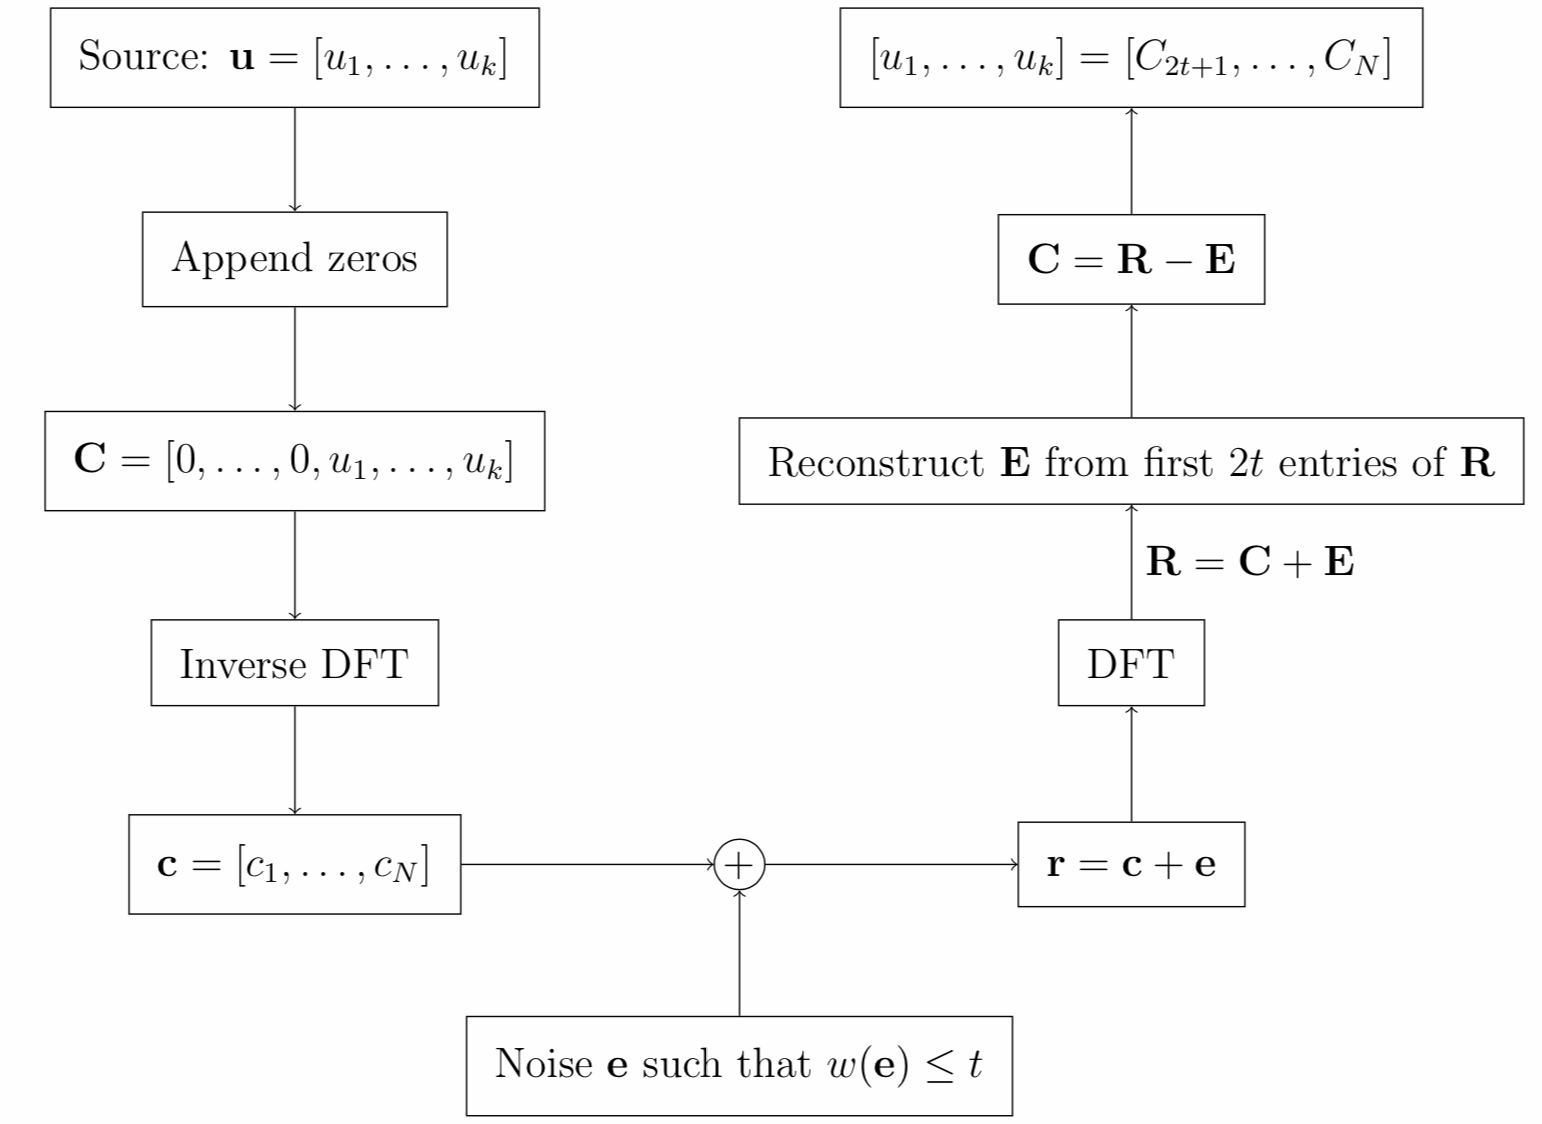
\includegraphics[width=0.8\textwidth]{figs/reed-solomon}
\end{figure}
Note that Blahut's Theorem is essential; the first $2t$ entries of $\vect{R}$ correspond to the error vector only, and since the weight of $\vect{e} \leq t$, the linear complexity of $\vect{E} \leq t$. 

\ix{The Parity Check Matrix}$\vect{H}$ consists of the first $2t = N-K$ rows (or columns, since symmetric) of the DFT matrix, since any $\vect{c}$ must have zeros in the first $2t$ positions once decoded. 

\ix{The Encoder Matrix}The encoder matrix, $\vect{G}$, is the last $N - 2t$ rows of the inverse DFT matrix (the first $2t$ rows are not used due to the zero padding. A systematic encoder can be created by performing elementary row operations on $\vect{G}$ to bring it into systematic form. The above scheme is then modified by removing the inverse DFT on the transmitted and instead applying the inverse DFT to $\vect{C}$, then outputting the systematic part only. The first $2t$ entries of $\vect{R}$ correspond to $\vect{e}$ only still as the elementary row operations change the terms in $\vect{C}$ corresponding only to the $u$. 

\ix{MDS}A Reed-Solomon code can correct $t$ errors when $N-K = 2t$. Therefore, the minimum distance must be greater than $2t + 1$, \textbf{which fufils the Singleton bound with equality}. 

\chapter{Introduction to Cryptology}
\section{Introduction}
\emph{Cryptanalysis} aims to find out the secrets which have been hidden using cryptographic methods. Cryptanalysis can attempt to do this in a number of ways\ix{Cryptanalysis Attacks}:
\begin{enumerate}
	\item Ciphertext only attack: the cryptanalyst has access to the ciphertext only. 
	\item Known plaintext attack: the cryptanalyst has access to a plaintext ciphertext pair. 
	\item Chosen plaintext attack: the cryptanalyst can \emph{choose} the plaintext to be encrypted. This is common in modern attacks where the enemy cryptanalysis use impersonation. 
	\item Chosen ciphertext attack: the cryptanalyst can cause chosen encrypted messages to be decrypted. 
\end{enumerate}

\ix{Aims of Cryptography}\emph{Cryptography} aims to ensure both \emph{secrecy} (ensuring that only the intended recipient can read the message) and \emph{authenticity} (ensuring the reader is confident about the message author) between communication parties. These aims are dual, and protocols exist that satisfy one but not the other. Often, two processes may be required to ensure that both aims are met. Cryptosystems are classified according to a number of criteria. 

\ix{Cryptosystems: Key Types}\emph{Secret key cryptosystems} rely on the existence between a shared secret key known only to origin and destination whilst \emph{public key cryptosystems} do not assume the existence of this key, and aim to establish a secret channel in full view of the enemy cryptanalyst. These techniques rely on the availability of authenticity to guarantee secrecy.  

\ix{Security}\emph{Unconditional security} concerns itself with methods for which there are mathematical proofs of safety (and thus the enemy cryptanalyst could be unlimited computational resources). \emph{Computational security} concerns itself with algorithms that ensure security against \textbf{adversaries with limited computational resources, using all currently known and published mathematical knowledge}. Most practical methods are computationally secure, though there has been an increasing research focus on unconditional security. 

\begin{principle}[Kerchkoff's Principle]
	\ix{Kerchoff's Principle}The cipher should be designed to be secure when the enemy cryptanalyst knows all details of the enciphering process and deciphering process \textbf{except the secret key}. 
\end{principle}

\section{Public Key Cryptography}
\ix{Trapdoor One-Way Functions}Public key cryptography relies on the concept of \emph{one-way functions} which can be computed in one direction easily but whose inverse is very hard to compute or \emph{trapdoor one-way functions} which are similar, but whose inverse can be computed easily if one knows the secret `trapdoor', typically a secret number. 

\subsection{The Diffie Hellman Key Distribution System }
Let $\alpha$ be the generator for a cyclic group. It is difficult to invert discrete exponentiation, $\alpha^x$, for an unknown $x$\ix{One-Way Function} for groups whose order has a large prime factor e.g. $\text{GF}(p)$ where $p-1$ has a large prime factor. The inversion is known as the \emph{discrete logarithm} which satisfies the usual properties of logarithms:
\begin{align}
\log_\alpha(n_1 \odot n_2) &= \log_\alpha n_1 \oplus \log_\alpha n_2 \\
\log_\alpha(n_1^{n_2}) &= n_2 \odot \log_\alpha n_1
\end{align}
\begin{figure}[H]
	\centering
	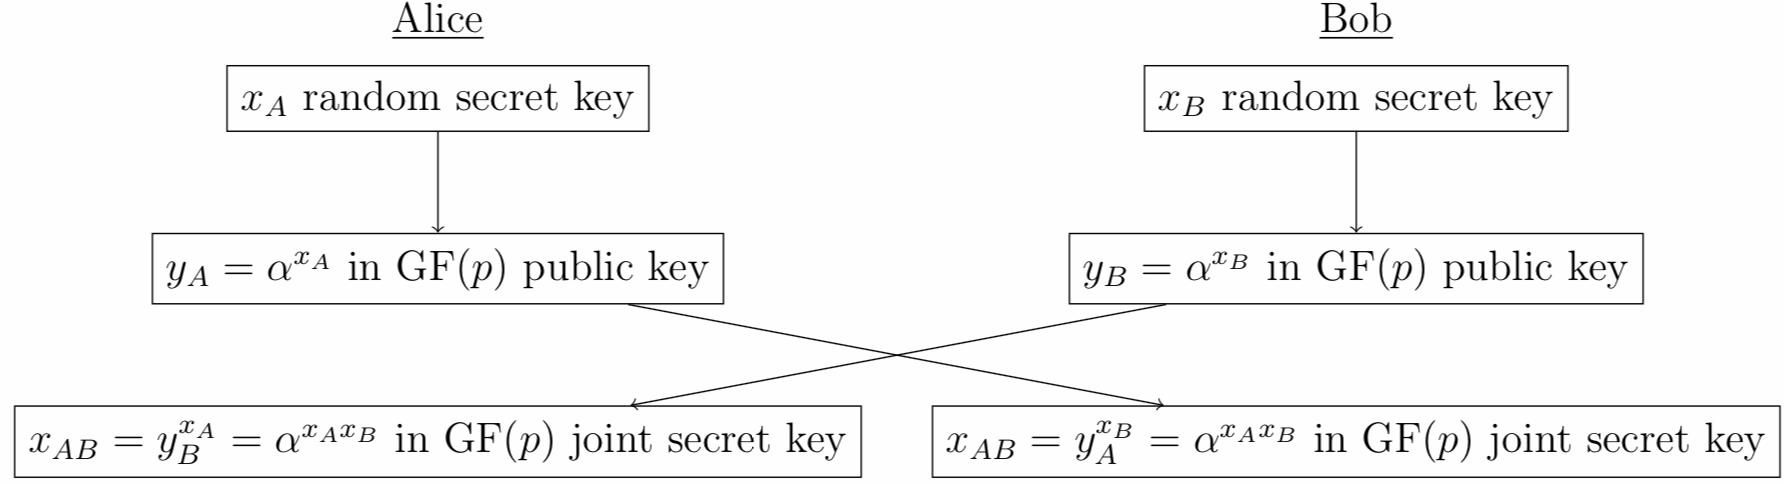
\includegraphics[width=\textwidth]{figs/diffie-hellman}
\end{figure}
\ix{Components of the Diffie Hellman System}The system components are:
\begin{enumerate}[label=(\alph*):]
	\item Modulus $p$ and generator $\alpha$: published and define the system. 
	\item Secret keys $x_A$ and $x_B$. Chosen using a strong random number generator.\ix{Caveat} Note that if the random number generation is not strong (i.e. not truly random), this protocol is vulnerable to attacks. 
	\item Public keys $y_A = \alpha^{x_A}$ and $y_B = \alpha^{x_B}$. Fully accessible to all parties.\ix{Practical Consideration} In practice, a trusted authentication authority is requires to publish keys in a manner that cannot be tampered with and vouches for their authenticity. 
	\item Joint secret key $\alpha^{x_A x_B}$. 
\end{enumerate}
This technique allows Alice and Bob to agree on a secret key which is known only to them and relies on the difficulty of computing the discrete logarithm. 

\subsection{The Rivest-Shamir-Adelman Public-Key Cryptosystem}
RSA is an encryption protocol which relies on the difficulty to factoring a large number, $m$, into it's prime factors. 
\ix{RSA Schematic}
\begin{figure}[H]
	\centering
	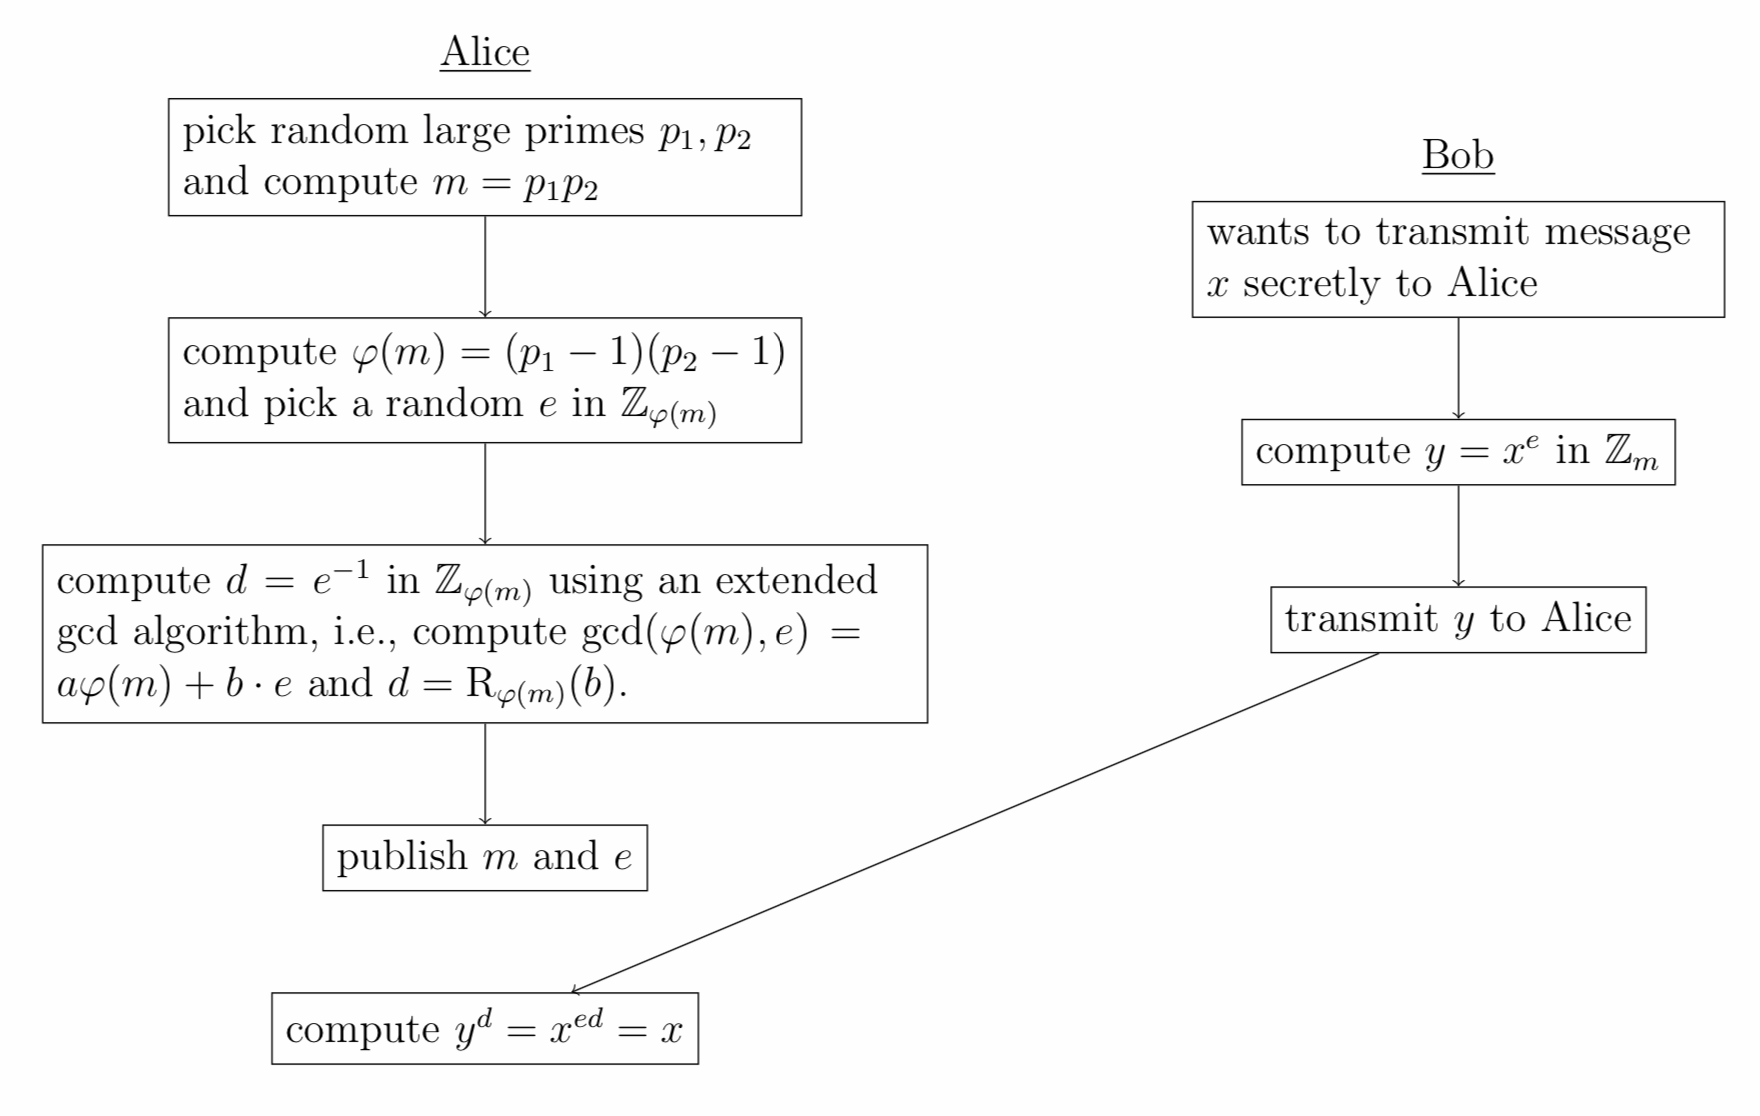
\includegraphics[width=\textwidth]{figs/RSA}
\end{figure}
Note that when operating in $\mathbb{Z}_m$, operations in the exponent occur modulo $\varphi(m)$ i.e.:
\begin{align}
x^{e_1} \odot_m x^{e_2} &= x^{e_1 \oplus_{\varphi(m)} e_2 } \\
(x^{e_1})^{e_2} &= x^{e_1 \odot_{\varphi(m)} e_2}
\end{align}
Only somebody who knows $\varphi(m)$ (which can be obtained by the secret prime) can find $d = e^{-1}$ in $\mathbb{Z}_{\varphi(m)}$ and hence invert the operation $x^{e}$ in $\mathbb{Z}^m$. The protocol enables Alice to publish a public key which allows anyone to transmit messages that only Alice can read. \ix{Real World Consideration}In reality, it is essential that the public key is published in a manner that it cannot be tampered with.\ix{System Components}The components of the system are:
\begin{enumerate}[label=(\alph*):]
	\item Secret keys $p_1, p_2$ which are the initial secrets which must be chosen using reliable, unpredictable generators of large random primes; predictability can reduce the search space in an attack.
	\item The published key, $m = p_1 p_2$ and $e$. $e$ must be invertible in $\mathbb{Z}_{\varphi(m)}$.\ix{Generating $e$} It could be generated using the CRT if a factor of $\varphi(m)$ is available. 
	\item Alice's generated secrets are $\varphi(m)$ and $d$. $d$ is computed using an extended GCD algorithm such as Stein's extended algorithm. 
\end{enumerate}
Note that RSA also relies on the difficulty of computing the discrete logarithm; in a known plaintext attack, the adversary could compute $d = \log_y x$. 

\subsection*{RSA Works for Any $x$}
In this section, we show that RSA decryption works for any value of $x$. The modulo used is:
\begin{align}
m = p_1 p_2 \hspace{1cm} \varphi(m) = (1 - p_1) (1 - p_2)
\end{align}
We choose $e, d$ such that $e \odot_{\varphi(m)} d = 1$. Therefore:
\begin{align}
ed - k \varphi(m) = ed - k (p_1 - 1) (p_2 - 1) = 1
\end{align}
Therefore:
\begin{align}
e \odot_{p_1-1} d = 1 \text{ and } e \odot_{p_2-1} d = 1
\end{align}
A message, $x \in \mathbb{Z}_m$, is chosen and encrypted using $y = R_{m}(x^e)$. The decoding rule is $\tilde{x} = R_{m}(y^d)$.
\begin{align}
\tilde{x} = R_m(y^d) = R_m(R_m(x^e)^d) = R_m(x^{ed})
\end{align}
Note that $e \odot_x d = 1 \Leftrightarrow ed - kx = 1$. Now, consider:
\begin{align}
x^{ed} &= x^{1 + k(p_1 - 1)} \nonumber\\
&= x (x^{p_1 - 1})^k \nonumber\\
&= x (x^{p_2 - 1})^k
\end{align}
Fermat's Theorem implies that:
\begin{align}
R_{p_1}(x^{ed} - x) &= R_{p_1}(R_{p_1}(x) \cdot  \underbrace{R_{p_1}(x^{p_1 - 1})^k}_{1} - R_{p_1}(x) ) \nonumber \\
&= R_{p_1}(x - x) \nonumber\\
&= 0
\end{align}
Similarily, $R_{p_2}(x^{ed} - x) = 0$. Therefore,
\begin{align}
x^{ed} - x = k p_1 p_2 = k m
\end{align}
Therefore:
\begin{align}
R_m(\tilde{x} - x) = 0
\end{align}


\end{document}